
% Default to the notebook output style

    


% Inherit from the specified cell style.




    
\documentclass[11pt]{article}

    
    
    \usepackage[T1]{fontenc}
    % Nicer default font (+ math font) than Computer Modern for most use cases
    \usepackage{mathpazo}

    % Basic figure setup, for now with no caption control since it's done
    % automatically by Pandoc (which extracts ![](path) syntax from Markdown).
    \usepackage{graphicx}
    % We will generate all images so they have a width \maxwidth. This means
    % that they will get their normal width if they fit onto the page, but
    % are scaled down if they would overflow the margins.
    \makeatletter
    \def\maxwidth{\ifdim\Gin@nat@width>\linewidth\linewidth
    \else\Gin@nat@width\fi}
    \makeatother
    \let\Oldincludegraphics\includegraphics
    % Set max figure width to be 80% of text width, for now hardcoded.
    \renewcommand{\includegraphics}[1]{\Oldincludegraphics[width=.8\maxwidth]{#1}}
    % Ensure that by default, figures have no caption (until we provide a
    % proper Figure object with a Caption API and a way to capture that
    % in the conversion process - todo).
    \usepackage{caption}
    \DeclareCaptionLabelFormat{nolabel}{}
    \captionsetup{labelformat=nolabel}

    \usepackage{adjustbox} % Used to constrain images to a maximum size 
    \usepackage{xcolor} % Allow colors to be defined
    \usepackage{enumerate} % Needed for markdown enumerations to work
    \usepackage{geometry} % Used to adjust the document margins
    \usepackage{amsmath} % Equations
    \usepackage{amssymb} % Equations
    \usepackage{textcomp} % defines textquotesingle
    % Hack from http://tex.stackexchange.com/a/47451/13684:
    \AtBeginDocument{%
        \def\PYZsq{\textquotesingle}% Upright quotes in Pygmentized code
    }
    \usepackage{upquote} % Upright quotes for verbatim code
    \usepackage{eurosym} % defines \euro
    \usepackage[mathletters]{ucs} % Extended unicode (utf-8) support
    \usepackage[utf8x]{inputenc} % Allow utf-8 characters in the tex document
    \usepackage{fancyvrb} % verbatim replacement that allows latex
    \usepackage{grffile} % extends the file name processing of package graphics 
                         % to support a larger range 
    % The hyperref package gives us a pdf with properly built
    % internal navigation ('pdf bookmarks' for the table of contents,
    % internal cross-reference links, web links for URLs, etc.)
    \usepackage{hyperref}
    \usepackage{longtable} % longtable support required by pandoc >1.10
    \usepackage{booktabs}  % table support for pandoc > 1.12.2
    \usepackage[inline]{enumitem} % IRkernel/repr support (it uses the enumerate* environment)
    \usepackage[normalem]{ulem} % ulem is needed to support strikethroughs (\sout)
                                % normalem makes italics be italics, not underlines
    

    
    
    % Colors for the hyperref package
    \definecolor{urlcolor}{rgb}{0,.145,.698}
    \definecolor{linkcolor}{rgb}{.71,0.21,0.01}
    \definecolor{citecolor}{rgb}{.12,.54,.11}

    % ANSI colors
    \definecolor{ansi-black}{HTML}{3E424D}
    \definecolor{ansi-black-intense}{HTML}{282C36}
    \definecolor{ansi-red}{HTML}{E75C58}
    \definecolor{ansi-red-intense}{HTML}{B22B31}
    \definecolor{ansi-green}{HTML}{00A250}
    \definecolor{ansi-green-intense}{HTML}{007427}
    \definecolor{ansi-yellow}{HTML}{DDB62B}
    \definecolor{ansi-yellow-intense}{HTML}{B27D12}
    \definecolor{ansi-blue}{HTML}{208FFB}
    \definecolor{ansi-blue-intense}{HTML}{0065CA}
    \definecolor{ansi-magenta}{HTML}{D160C4}
    \definecolor{ansi-magenta-intense}{HTML}{A03196}
    \definecolor{ansi-cyan}{HTML}{60C6C8}
    \definecolor{ansi-cyan-intense}{HTML}{258F8F}
    \definecolor{ansi-white}{HTML}{C5C1B4}
    \definecolor{ansi-white-intense}{HTML}{A1A6B2}

    % commands and environments needed by pandoc snippets
    % extracted from the output of `pandoc -s`
    \providecommand{\tightlist}{%
      \setlength{\itemsep}{0pt}\setlength{\parskip}{0pt}}
    \DefineVerbatimEnvironment{Highlighting}{Verbatim}{commandchars=\\\{\}}
    % Add ',fontsize=\small' for more characters per line
    \newenvironment{Shaded}{}{}
    \newcommand{\KeywordTok}[1]{\textcolor[rgb]{0.00,0.44,0.13}{\textbf{{#1}}}}
    \newcommand{\DataTypeTok}[1]{\textcolor[rgb]{0.56,0.13,0.00}{{#1}}}
    \newcommand{\DecValTok}[1]{\textcolor[rgb]{0.25,0.63,0.44}{{#1}}}
    \newcommand{\BaseNTok}[1]{\textcolor[rgb]{0.25,0.63,0.44}{{#1}}}
    \newcommand{\FloatTok}[1]{\textcolor[rgb]{0.25,0.63,0.44}{{#1}}}
    \newcommand{\CharTok}[1]{\textcolor[rgb]{0.25,0.44,0.63}{{#1}}}
    \newcommand{\StringTok}[1]{\textcolor[rgb]{0.25,0.44,0.63}{{#1}}}
    \newcommand{\CommentTok}[1]{\textcolor[rgb]{0.38,0.63,0.69}{\textit{{#1}}}}
    \newcommand{\OtherTok}[1]{\textcolor[rgb]{0.00,0.44,0.13}{{#1}}}
    \newcommand{\AlertTok}[1]{\textcolor[rgb]{1.00,0.00,0.00}{\textbf{{#1}}}}
    \newcommand{\FunctionTok}[1]{\textcolor[rgb]{0.02,0.16,0.49}{{#1}}}
    \newcommand{\RegionMarkerTok}[1]{{#1}}
    \newcommand{\ErrorTok}[1]{\textcolor[rgb]{1.00,0.00,0.00}{\textbf{{#1}}}}
    \newcommand{\NormalTok}[1]{{#1}}
    
    % Additional commands for more recent versions of Pandoc
    \newcommand{\ConstantTok}[1]{\textcolor[rgb]{0.53,0.00,0.00}{{#1}}}
    \newcommand{\SpecialCharTok}[1]{\textcolor[rgb]{0.25,0.44,0.63}{{#1}}}
    \newcommand{\VerbatimStringTok}[1]{\textcolor[rgb]{0.25,0.44,0.63}{{#1}}}
    \newcommand{\SpecialStringTok}[1]{\textcolor[rgb]{0.73,0.40,0.53}{{#1}}}
    \newcommand{\ImportTok}[1]{{#1}}
    \newcommand{\DocumentationTok}[1]{\textcolor[rgb]{0.73,0.13,0.13}{\textit{{#1}}}}
    \newcommand{\AnnotationTok}[1]{\textcolor[rgb]{0.38,0.63,0.69}{\textbf{\textit{{#1}}}}}
    \newcommand{\CommentVarTok}[1]{\textcolor[rgb]{0.38,0.63,0.69}{\textbf{\textit{{#1}}}}}
    \newcommand{\VariableTok}[1]{\textcolor[rgb]{0.10,0.09,0.49}{{#1}}}
    \newcommand{\ControlFlowTok}[1]{\textcolor[rgb]{0.00,0.44,0.13}{\textbf{{#1}}}}
    \newcommand{\OperatorTok}[1]{\textcolor[rgb]{0.40,0.40,0.40}{{#1}}}
    \newcommand{\BuiltInTok}[1]{{#1}}
    \newcommand{\ExtensionTok}[1]{{#1}}
    \newcommand{\PreprocessorTok}[1]{\textcolor[rgb]{0.74,0.48,0.00}{{#1}}}
    \newcommand{\AttributeTok}[1]{\textcolor[rgb]{0.49,0.56,0.16}{{#1}}}
    \newcommand{\InformationTok}[1]{\textcolor[rgb]{0.38,0.63,0.69}{\textbf{\textit{{#1}}}}}
    \newcommand{\WarningTok}[1]{\textcolor[rgb]{0.38,0.63,0.69}{\textbf{\textit{{#1}}}}}
    
    
    % Define a nice break command that doesn't care if a line doesn't already
    % exist.
    \def\br{\hspace*{\fill} \\* }
    % Math Jax compatability definitions
    \def\gt{>}
    \def\lt{<}
    % Document parameters
    \title{Capstone\_3-22-2019}
    
    
    

    % Pygments definitions
    
\makeatletter
\def\PY@reset{\let\PY@it=\relax \let\PY@bf=\relax%
    \let\PY@ul=\relax \let\PY@tc=\relax%
    \let\PY@bc=\relax \let\PY@ff=\relax}
\def\PY@tok#1{\csname PY@tok@#1\endcsname}
\def\PY@toks#1+{\ifx\relax#1\empty\else%
    \PY@tok{#1}\expandafter\PY@toks\fi}
\def\PY@do#1{\PY@bc{\PY@tc{\PY@ul{%
    \PY@it{\PY@bf{\PY@ff{#1}}}}}}}
\def\PY#1#2{\PY@reset\PY@toks#1+\relax+\PY@do{#2}}

\expandafter\def\csname PY@tok@w\endcsname{\def\PY@tc##1{\textcolor[rgb]{0.73,0.73,0.73}{##1}}}
\expandafter\def\csname PY@tok@c\endcsname{\let\PY@it=\textit\def\PY@tc##1{\textcolor[rgb]{0.25,0.50,0.50}{##1}}}
\expandafter\def\csname PY@tok@cp\endcsname{\def\PY@tc##1{\textcolor[rgb]{0.74,0.48,0.00}{##1}}}
\expandafter\def\csname PY@tok@k\endcsname{\let\PY@bf=\textbf\def\PY@tc##1{\textcolor[rgb]{0.00,0.50,0.00}{##1}}}
\expandafter\def\csname PY@tok@kp\endcsname{\def\PY@tc##1{\textcolor[rgb]{0.00,0.50,0.00}{##1}}}
\expandafter\def\csname PY@tok@kt\endcsname{\def\PY@tc##1{\textcolor[rgb]{0.69,0.00,0.25}{##1}}}
\expandafter\def\csname PY@tok@o\endcsname{\def\PY@tc##1{\textcolor[rgb]{0.40,0.40,0.40}{##1}}}
\expandafter\def\csname PY@tok@ow\endcsname{\let\PY@bf=\textbf\def\PY@tc##1{\textcolor[rgb]{0.67,0.13,1.00}{##1}}}
\expandafter\def\csname PY@tok@nb\endcsname{\def\PY@tc##1{\textcolor[rgb]{0.00,0.50,0.00}{##1}}}
\expandafter\def\csname PY@tok@nf\endcsname{\def\PY@tc##1{\textcolor[rgb]{0.00,0.00,1.00}{##1}}}
\expandafter\def\csname PY@tok@nc\endcsname{\let\PY@bf=\textbf\def\PY@tc##1{\textcolor[rgb]{0.00,0.00,1.00}{##1}}}
\expandafter\def\csname PY@tok@nn\endcsname{\let\PY@bf=\textbf\def\PY@tc##1{\textcolor[rgb]{0.00,0.00,1.00}{##1}}}
\expandafter\def\csname PY@tok@ne\endcsname{\let\PY@bf=\textbf\def\PY@tc##1{\textcolor[rgb]{0.82,0.25,0.23}{##1}}}
\expandafter\def\csname PY@tok@nv\endcsname{\def\PY@tc##1{\textcolor[rgb]{0.10,0.09,0.49}{##1}}}
\expandafter\def\csname PY@tok@no\endcsname{\def\PY@tc##1{\textcolor[rgb]{0.53,0.00,0.00}{##1}}}
\expandafter\def\csname PY@tok@nl\endcsname{\def\PY@tc##1{\textcolor[rgb]{0.63,0.63,0.00}{##1}}}
\expandafter\def\csname PY@tok@ni\endcsname{\let\PY@bf=\textbf\def\PY@tc##1{\textcolor[rgb]{0.60,0.60,0.60}{##1}}}
\expandafter\def\csname PY@tok@na\endcsname{\def\PY@tc##1{\textcolor[rgb]{0.49,0.56,0.16}{##1}}}
\expandafter\def\csname PY@tok@nt\endcsname{\let\PY@bf=\textbf\def\PY@tc##1{\textcolor[rgb]{0.00,0.50,0.00}{##1}}}
\expandafter\def\csname PY@tok@nd\endcsname{\def\PY@tc##1{\textcolor[rgb]{0.67,0.13,1.00}{##1}}}
\expandafter\def\csname PY@tok@s\endcsname{\def\PY@tc##1{\textcolor[rgb]{0.73,0.13,0.13}{##1}}}
\expandafter\def\csname PY@tok@sd\endcsname{\let\PY@it=\textit\def\PY@tc##1{\textcolor[rgb]{0.73,0.13,0.13}{##1}}}
\expandafter\def\csname PY@tok@si\endcsname{\let\PY@bf=\textbf\def\PY@tc##1{\textcolor[rgb]{0.73,0.40,0.53}{##1}}}
\expandafter\def\csname PY@tok@se\endcsname{\let\PY@bf=\textbf\def\PY@tc##1{\textcolor[rgb]{0.73,0.40,0.13}{##1}}}
\expandafter\def\csname PY@tok@sr\endcsname{\def\PY@tc##1{\textcolor[rgb]{0.73,0.40,0.53}{##1}}}
\expandafter\def\csname PY@tok@ss\endcsname{\def\PY@tc##1{\textcolor[rgb]{0.10,0.09,0.49}{##1}}}
\expandafter\def\csname PY@tok@sx\endcsname{\def\PY@tc##1{\textcolor[rgb]{0.00,0.50,0.00}{##1}}}
\expandafter\def\csname PY@tok@m\endcsname{\def\PY@tc##1{\textcolor[rgb]{0.40,0.40,0.40}{##1}}}
\expandafter\def\csname PY@tok@gh\endcsname{\let\PY@bf=\textbf\def\PY@tc##1{\textcolor[rgb]{0.00,0.00,0.50}{##1}}}
\expandafter\def\csname PY@tok@gu\endcsname{\let\PY@bf=\textbf\def\PY@tc##1{\textcolor[rgb]{0.50,0.00,0.50}{##1}}}
\expandafter\def\csname PY@tok@gd\endcsname{\def\PY@tc##1{\textcolor[rgb]{0.63,0.00,0.00}{##1}}}
\expandafter\def\csname PY@tok@gi\endcsname{\def\PY@tc##1{\textcolor[rgb]{0.00,0.63,0.00}{##1}}}
\expandafter\def\csname PY@tok@gr\endcsname{\def\PY@tc##1{\textcolor[rgb]{1.00,0.00,0.00}{##1}}}
\expandafter\def\csname PY@tok@ge\endcsname{\let\PY@it=\textit}
\expandafter\def\csname PY@tok@gs\endcsname{\let\PY@bf=\textbf}
\expandafter\def\csname PY@tok@gp\endcsname{\let\PY@bf=\textbf\def\PY@tc##1{\textcolor[rgb]{0.00,0.00,0.50}{##1}}}
\expandafter\def\csname PY@tok@go\endcsname{\def\PY@tc##1{\textcolor[rgb]{0.53,0.53,0.53}{##1}}}
\expandafter\def\csname PY@tok@gt\endcsname{\def\PY@tc##1{\textcolor[rgb]{0.00,0.27,0.87}{##1}}}
\expandafter\def\csname PY@tok@err\endcsname{\def\PY@bc##1{\setlength{\fboxsep}{0pt}\fcolorbox[rgb]{1.00,0.00,0.00}{1,1,1}{\strut ##1}}}
\expandafter\def\csname PY@tok@kc\endcsname{\let\PY@bf=\textbf\def\PY@tc##1{\textcolor[rgb]{0.00,0.50,0.00}{##1}}}
\expandafter\def\csname PY@tok@kd\endcsname{\let\PY@bf=\textbf\def\PY@tc##1{\textcolor[rgb]{0.00,0.50,0.00}{##1}}}
\expandafter\def\csname PY@tok@kn\endcsname{\let\PY@bf=\textbf\def\PY@tc##1{\textcolor[rgb]{0.00,0.50,0.00}{##1}}}
\expandafter\def\csname PY@tok@kr\endcsname{\let\PY@bf=\textbf\def\PY@tc##1{\textcolor[rgb]{0.00,0.50,0.00}{##1}}}
\expandafter\def\csname PY@tok@bp\endcsname{\def\PY@tc##1{\textcolor[rgb]{0.00,0.50,0.00}{##1}}}
\expandafter\def\csname PY@tok@fm\endcsname{\def\PY@tc##1{\textcolor[rgb]{0.00,0.00,1.00}{##1}}}
\expandafter\def\csname PY@tok@vc\endcsname{\def\PY@tc##1{\textcolor[rgb]{0.10,0.09,0.49}{##1}}}
\expandafter\def\csname PY@tok@vg\endcsname{\def\PY@tc##1{\textcolor[rgb]{0.10,0.09,0.49}{##1}}}
\expandafter\def\csname PY@tok@vi\endcsname{\def\PY@tc##1{\textcolor[rgb]{0.10,0.09,0.49}{##1}}}
\expandafter\def\csname PY@tok@vm\endcsname{\def\PY@tc##1{\textcolor[rgb]{0.10,0.09,0.49}{##1}}}
\expandafter\def\csname PY@tok@sa\endcsname{\def\PY@tc##1{\textcolor[rgb]{0.73,0.13,0.13}{##1}}}
\expandafter\def\csname PY@tok@sb\endcsname{\def\PY@tc##1{\textcolor[rgb]{0.73,0.13,0.13}{##1}}}
\expandafter\def\csname PY@tok@sc\endcsname{\def\PY@tc##1{\textcolor[rgb]{0.73,0.13,0.13}{##1}}}
\expandafter\def\csname PY@tok@dl\endcsname{\def\PY@tc##1{\textcolor[rgb]{0.73,0.13,0.13}{##1}}}
\expandafter\def\csname PY@tok@s2\endcsname{\def\PY@tc##1{\textcolor[rgb]{0.73,0.13,0.13}{##1}}}
\expandafter\def\csname PY@tok@sh\endcsname{\def\PY@tc##1{\textcolor[rgb]{0.73,0.13,0.13}{##1}}}
\expandafter\def\csname PY@tok@s1\endcsname{\def\PY@tc##1{\textcolor[rgb]{0.73,0.13,0.13}{##1}}}
\expandafter\def\csname PY@tok@mb\endcsname{\def\PY@tc##1{\textcolor[rgb]{0.40,0.40,0.40}{##1}}}
\expandafter\def\csname PY@tok@mf\endcsname{\def\PY@tc##1{\textcolor[rgb]{0.40,0.40,0.40}{##1}}}
\expandafter\def\csname PY@tok@mh\endcsname{\def\PY@tc##1{\textcolor[rgb]{0.40,0.40,0.40}{##1}}}
\expandafter\def\csname PY@tok@mi\endcsname{\def\PY@tc##1{\textcolor[rgb]{0.40,0.40,0.40}{##1}}}
\expandafter\def\csname PY@tok@il\endcsname{\def\PY@tc##1{\textcolor[rgb]{0.40,0.40,0.40}{##1}}}
\expandafter\def\csname PY@tok@mo\endcsname{\def\PY@tc##1{\textcolor[rgb]{0.40,0.40,0.40}{##1}}}
\expandafter\def\csname PY@tok@ch\endcsname{\let\PY@it=\textit\def\PY@tc##1{\textcolor[rgb]{0.25,0.50,0.50}{##1}}}
\expandafter\def\csname PY@tok@cm\endcsname{\let\PY@it=\textit\def\PY@tc##1{\textcolor[rgb]{0.25,0.50,0.50}{##1}}}
\expandafter\def\csname PY@tok@cpf\endcsname{\let\PY@it=\textit\def\PY@tc##1{\textcolor[rgb]{0.25,0.50,0.50}{##1}}}
\expandafter\def\csname PY@tok@c1\endcsname{\let\PY@it=\textit\def\PY@tc##1{\textcolor[rgb]{0.25,0.50,0.50}{##1}}}
\expandafter\def\csname PY@tok@cs\endcsname{\let\PY@it=\textit\def\PY@tc##1{\textcolor[rgb]{0.25,0.50,0.50}{##1}}}

\def\PYZbs{\char`\\}
\def\PYZus{\char`\_}
\def\PYZob{\char`\{}
\def\PYZcb{\char`\}}
\def\PYZca{\char`\^}
\def\PYZam{\char`\&}
\def\PYZlt{\char`\<}
\def\PYZgt{\char`\>}
\def\PYZsh{\char`\#}
\def\PYZpc{\char`\%}
\def\PYZdl{\char`\$}
\def\PYZhy{\char`\-}
\def\PYZsq{\char`\'}
\def\PYZdq{\char`\"}
\def\PYZti{\char`\~}
% for compatibility with earlier versions
\def\PYZat{@}
\def\PYZlb{[}
\def\PYZrb{]}
\makeatother


    % Exact colors from NB
    \definecolor{incolor}{rgb}{0.0, 0.0, 0.5}
    \definecolor{outcolor}{rgb}{0.545, 0.0, 0.0}



    
    % Prevent overflowing lines due to hard-to-break entities
    \sloppy 
    % Setup hyperref package
    \hypersetup{
      breaklinks=true,  % so long urls are correctly broken across lines
      colorlinks=true,
      urlcolor=urlcolor,
      linkcolor=linkcolor,
      citecolor=citecolor,
      }
    % Slightly bigger margins than the latex defaults
    
    \geometry{verbose,tmargin=1in,bmargin=1in,lmargin=1in,rmargin=1in}
    
    

    \begin{document}
    
    
    \maketitle
    
    

    
    \subsection{Capstone:}\label{capstone}

\section{Utilizing Meteorological Data with Supervised Learning to
Predict Snowfall Amounts at Ski
Resort}\label{utilizing-meteorological-data-with-supervised-learning-to-predict-snowfall-amounts-at-ski-resort}

\textbf{By Dustin Rapp}

\subsection{-\/-}\label{section}

\subsection{Introduction}\label{introduction}

\begin{center}\rule{0.5\linewidth}{\linethickness}\end{center}

Complex terrain in mountainous areas often make predicting snowfall
difficult with prognostic weather models - especially on specific slopes
or mountainsides where extremely localized air flows may complicate such
forecasts. With accurate snow forecasts, ski resorts can optimize their
snowfall making, grooming, and snow removal operations. An accurate
short term snowfall forecast, even for a small segment of the mountain
may likely assist a ski resort's operation. The goal of this study is to
get a glimpse into the potential of utilizing a supervised learning
techniques with freely available surface and meteorological data to
predict snowfall on a slope at Copper Mountain Ski Resort in Colorado.
Copper Mountain Ski Resort may be especially interested in such
predictive models because of the unique access to government funded
meteorological data being recorded near or onsite to their resort.

The purpose of this report is to discuss to describe an assessment of an
Ordinary Least Squares Model (OLS) to predict snowfall totals over a 12
hour timespan, given meteorological conditions at the beginning of the
12 hour period. Hourly meteorological data was obtained from nearby
meteorological stations and upper air stations and was then processed
into model-friendly inputs. A linear regression analysis was then
performed on the data to determine which features may have most
predictive power. Two OLS analyses were then performed - one which only
utilized surface meteorological data and one which utilized surface and
upper air data. Finally, two similar assessmsents were performed using a
decision tree regressor algorithm.

\subsection{Data}\label{data}

The Copper Mountain ski resort is unique as there is an official SNOTEL
National Resources Conservation Service monitoring station the north
slope of Copper Mountain, where many popular ski runs are located.
SNOTEL is a telemetry automated system of snowpack and related climate
sensors in the Western United States. In addition to reporting hourly
snowfall amounts, it also records temperature. The Copper Mountain ski
resort is also has an Colorado Department of Transportation Automated
Weather Observing System (AWOS) which monitors a suite of hourly
variables near the top of Copper Mountain. Additionally, a National
Weather Service Automated Surface Observing Station (ASOS) is located in
Leadville, CO approximately 30 km to the northwest of Copper Mountain.
The SNOTEL si referencenced as SNOTEL, K

These three stations give a comprehensive meteorological dataset of
surface variables in the vicinity of the Copper Mountain Resort.
\textbf{Table 1} gives a listing of all surface level meteorological
variables by station. Hourly data for each station was downloaded for
years 2005-2017 from online sources. Data sources for each station are
found in \textbf{Table 2}. A map showing the Copper Mountain SNOTEL site
and the meteorological sites used in this assessment is also shown in
\textbf{Figure 1}

\textbf{Table 1 - Meteorological Variables by Station}

\begin{longtable}[]{@{}ccccc@{}}
\toprule
\begin{minipage}[b]{0.18\columnwidth}\centering\strut
\textbf{Station ID/Num}\strut
\end{minipage} & \begin{minipage}[b]{0.18\columnwidth}\centering\strut
\textbf{Station Type}\strut
\end{minipage} & \begin{minipage}[b]{0.17\columnwidth}\centering\strut
\textbf{Elevation}\strut
\end{minipage} & \begin{minipage}[b]{0.15\columnwidth}\centering\strut
\textbf{Variables}\strut
\end{minipage} & \begin{minipage}[b]{0.18\columnwidth}\centering\strut
\textbf{Data Source}\strut
\end{minipage}\tabularnewline
\midrule
\endhead
\begin{minipage}[t]{0.18\columnwidth}\centering\strut
\textbf{SNOTEL 415}\strut
\end{minipage} & \begin{minipage}[t]{0.18\columnwidth}\centering\strut
SNOTEL\strut
\end{minipage} & \begin{minipage}[t]{0.17\columnwidth}\centering\strut
10550'\strut
\end{minipage} & \begin{minipage}[t]{0.15\columnwidth}\centering\strut
Temperature Snow Depth\strut
\end{minipage} & \begin{minipage}[t]{0.18\columnwidth}\centering\strut
National Resources Conservation Service (www.NRCS.gov)\strut
\end{minipage}\tabularnewline
\begin{minipage}[t]{0.18\columnwidth}\centering\strut
\textbf{KLXV}\strut
\end{minipage} & \begin{minipage}[t]{0.18\columnwidth}\centering\strut
ASOS\strut
\end{minipage} & \begin{minipage}[t]{0.17\columnwidth}\centering\strut
12075\strut
\end{minipage} & \begin{minipage}[t]{0.15\columnwidth}\centering\strut
Wind Speed Wind Direction Cloud Cover\strut
\end{minipage} & \begin{minipage}[t]{0.18\columnwidth}\centering\strut
National Climatic Data Center ISHD Lite format (www.NCDC.gov)\strut
\end{minipage}\tabularnewline
\begin{minipage}[t]{0.18\columnwidth}\centering\strut
\textbf{KCCU}\strut
\end{minipage} & \begin{minipage}[t]{0.18\columnwidth}\centering\strut
AWOS\strut
\end{minipage} & \begin{minipage}[t]{0.17\columnwidth}\centering\strut
10550'\strut
\end{minipage} & \begin{minipage}[t]{0.15\columnwidth}\centering\strut
Dewpoint W Wind Speed Wind Direction Cloud Cover\strut
\end{minipage} & \begin{minipage}[t]{0.18\columnwidth}\centering\strut
National Climatic Data Center ISHD Lite format (www.NCDC.gov)\strut
\end{minipage}\tabularnewline
\begin{minipage}[t]{0.18\columnwidth}\centering\strut
\textbf{KJCT}\strut
\end{minipage} & \begin{minipage}[t]{0.18\columnwidth}\centering\strut
RAOB\strut
\end{minipage} & \begin{minipage}[t]{0.17\columnwidth}\centering\strut
n/a\strut
\end{minipage} & \begin{minipage}[t]{0.15\columnwidth}\centering\strut
\strut
\end{minipage}\tabularnewline
\bottomrule
\end{longtable}

\begin{center}\rule{0.5\linewidth}{\linethickness}\end{center}

\begin{center}\rule{0.5\linewidth}{\linethickness}\end{center}

\textbf{Figure 1 - Map of SNOTEL and KCCU Station Locations at Copper
Mountain Ski Report}

\begin{longtable}[]{@{}lc@{}}
\toprule
\begin{minipage}[b]{0.39\columnwidth}\raggedright\strut
KXLV site relative to Copper Mountain Ski Resort\strut
\end{minipage} & \begin{minipage}[b]{0.55\columnwidth}\centering\strut
Relative locations of the SNOTEL and KCCU sites at the Copper Mountain
Ski Resort\strut
\end{minipage}\tabularnewline
\midrule
\endhead
\begin{minipage}[t]{0.39\columnwidth}\raggedright\strut
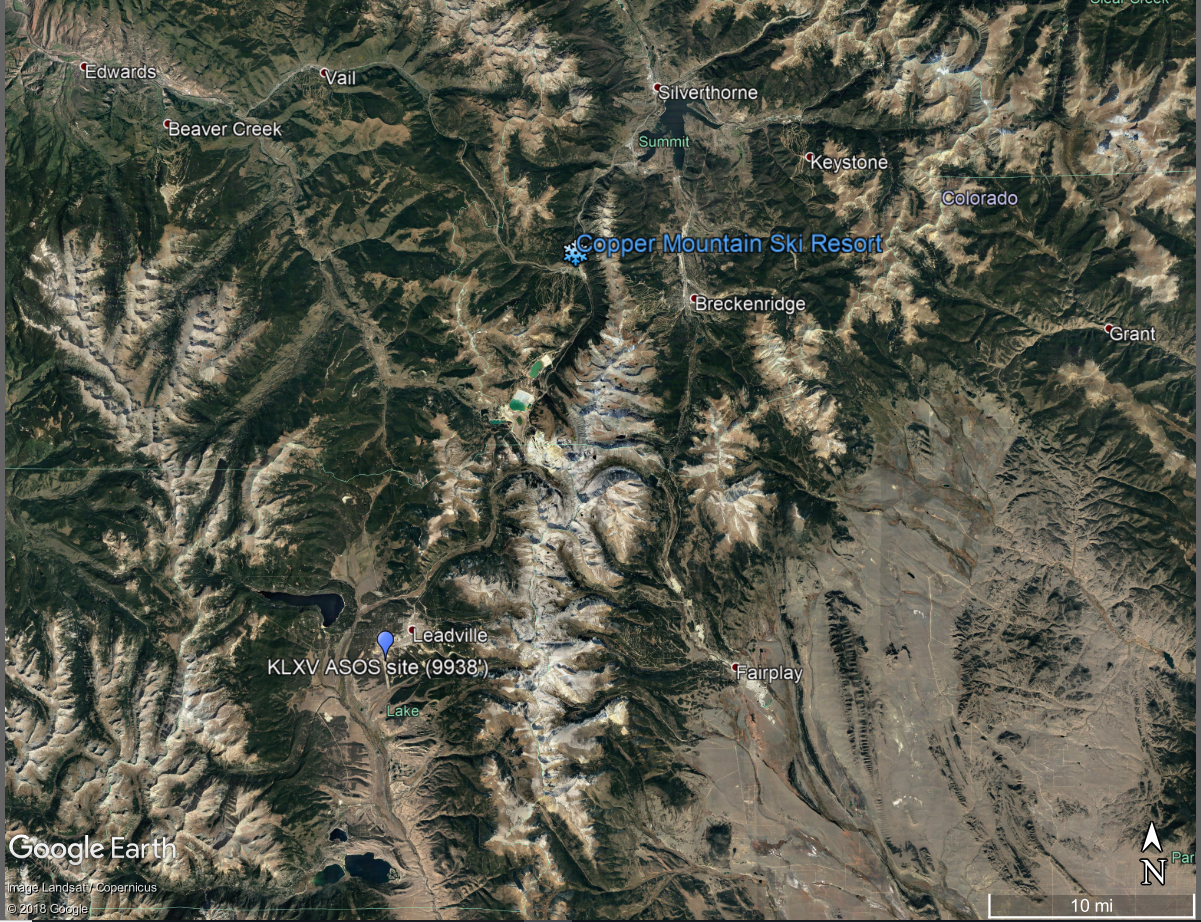
\includegraphics{figs/KLXV.png}\strut
\end{minipage} & \begin{minipage}[t]{0.55\columnwidth}\centering\strut
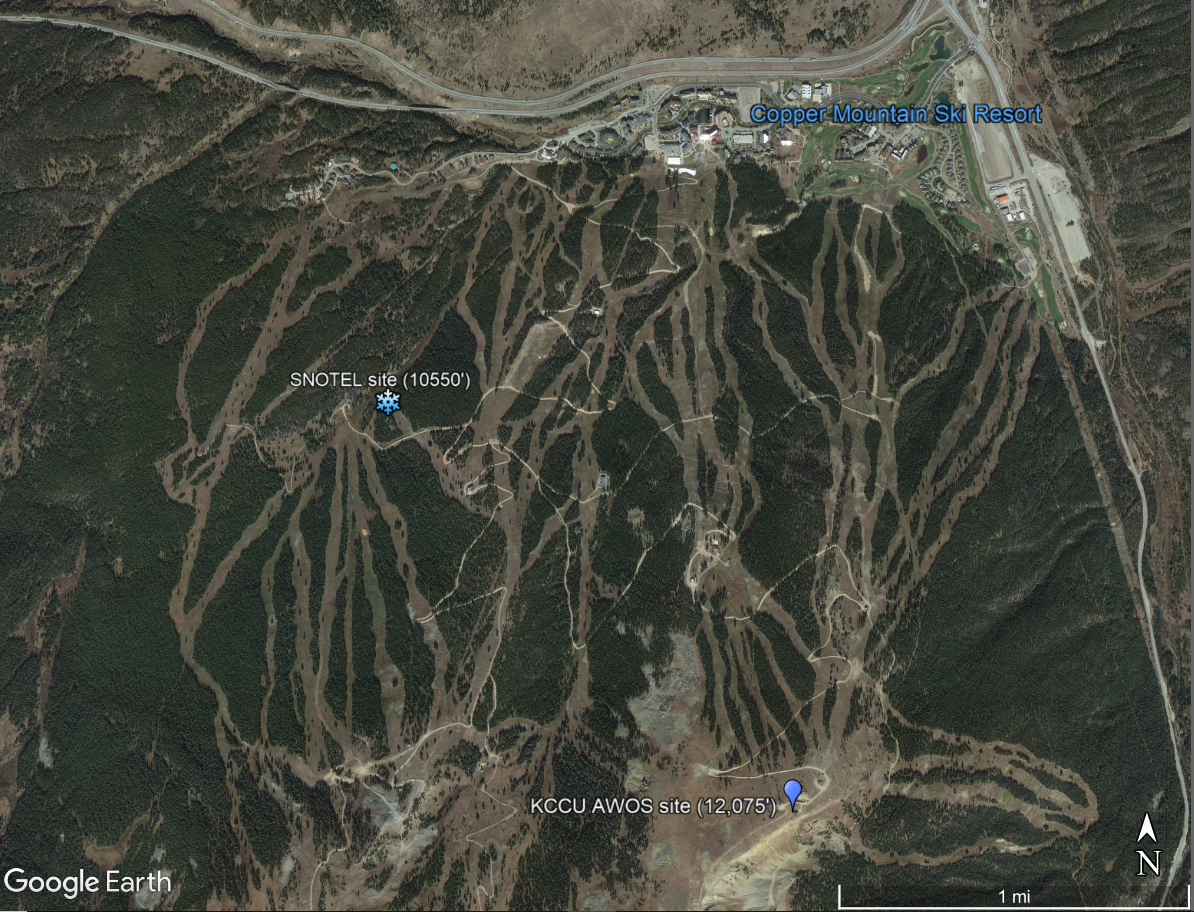
\includegraphics{figs/KCCU_and_SNOTEL_map.png}\strut
\end{minipage}\tabularnewline
\bottomrule
\end{longtable}

\subsection{Data and Wrangling
Cleaning}\label{data-and-wrangling-cleaning}

\subsubsection{Data Organization}\label{data-organization}

Hourly surface data from each station, downloaded, organized and
combined into a single timeseries dataframes with UTM timestamps.

The following cleanup steps were performed on this dataset:

\begin{itemize}
\tightlist
\item
  While the KCCU and KXLV datasets were already in UTM time, the NRCS
  dataset was in local time and required conversion to UTM.\\
\item
  The KCCU and KXLV datasets are in the Integrated Surface Hourly Data
  (ISHD) format and did require some manipulation (e.g. divided by 10)
  to get values into typical units.
\item
  Missing values (e.g. 9999 values) were translated to NaN values.
\item
  Missing data for all variables was linearly interpolated for time
  periods where 3 hours or less of data was missing.
\end{itemize}

The data was plotted to see if there were any extreme values warranting
removal. It was noted that some of the KCCU data (especially
temperature) did not demonstrate as much of a diurnal variation as the
KXLV station. These data are considered suspicious but were not removed
from the dataset. A more robust quality control of this dataset is
outside the scope of this preliminary study, but should be considered
for future studies.

A small amount of anomalous data was observed in the SNOTEL snow depth
data and was removed. These physically unrealistic readings (e.g. spikes
in some of the snow depth data or snowdepth reports which occur when
temperatures did not support snowfall) were removed as well as extreme
negative values.

\subsubsection{Additional Calculations}\label{additional-calculations}

\textbf{Pressure}\\
Changes in pressure are often a predictive indicator of weather
conditions (i.e. pressure drops often accompany strong storm systems), a
twelve hour pressure change variable was added to the datset. This was
calculated by subtracting the 00:00 observation from the upcoming 12:00
observation.

\textbf{Snowfall}\\
As the SNOTEL data only includes snow depth data instead of snowfall
data, snowfall was calculated based on changes in snowdepth. Due to the
sensitivity of the SNOTEL snow depth measurement sensors to external
forces (e.g. debris, air pressure), snow depth data from the SNOTEL site
appeared noisy for smaller snowstorms (i.e. less then 3 inches). To
minimize the small scale perturbations found in the data, 12 hour
snowfall totals were estimated at 00:00 UTC and 12:00 UTC and only 12-hr
snowfall events where greater then or equal to 3 inches occurred were
considered a snowfall event. The snowfall data was then added to
meteorological dataframe.

Because only 00:00 and 12:00 snowfall observations were utilized in the
analysis, all variables in the meteorological dataframe were reduced
from hourly observations to twelve hour observations. A new dataframe
was created utilizing only 00:00 and 12:00 observations.

A table showing the total number of snowfall events, along with mean,
max, and standard deviation of snowfall for each year is found in
\textbf{Table 3}. A timeseries plot showing the snowdepth, along with
these snowfall events is found in \textbf{Figure 2}.

\begin{center}\rule{0.5\linewidth}{\linethickness}\end{center}

\textbf{Table 3 Annual Statistics of 12-hr Snowfall Events
(\textgreater{}=3")}

\begin{center}\rule{0.5\linewidth}{\linethickness}\end{center}

\textbf{Insert Figure 2 Timeseries of snow depth and snowfall events}

\subsection{Data For Analysis}\label{data-for-analysis}

\begin{longtable}[]{@{}lllllll@{}}
\toprule
\begin{minipage}[b]{0.07\columnwidth}\raggedright\strut
Year\strut
\end{minipage} & \begin{minipage}[b]{0.34\columnwidth}\raggedright\strut
Number 12hr Snowfall Events \textgreater{}=3" with no missing
meteorological features missing for hour\strut
\end{minipage} & \begin{minipage}[b]{0.07\columnwidth}\raggedright\strut
Poss\strut
\end{minipage} & \begin{minipage}[b]{0.07\columnwidth}\raggedright\strut
Mean\strut
\end{minipage} & \begin{minipage}[b]{0.08\columnwidth}\raggedright\strut
Median\strut
\end{minipage} & \begin{minipage}[b]{0.06\columnwidth}\raggedright\strut
Max\strut
\end{minipage} & \begin{minipage}[b]{0.13\columnwidth}\raggedright\strut
Std Deviation\strut
\end{minipage}\tabularnewline
\midrule
\endhead
\begin{minipage}[t]{0.07\columnwidth}\raggedright\strut
2006\strut
\end{minipage} & \begin{minipage}[t]{0.34\columnwidth}\raggedright\strut
21\strut
\end{minipage} & \begin{minipage}[t]{0.07\columnwidth}\raggedright\strut
26\strut
\end{minipage} & \begin{minipage}[t]{0.07\columnwidth}\raggedright\strut
5\strut
\end{minipage} & \begin{minipage}[t]{0.08\columnwidth}\raggedright\strut
5\strut
\end{minipage} & \begin{minipage}[t]{0.06\columnwidth}\raggedright\strut
11\strut
\end{minipage} & \begin{minipage}[t]{0.13\columnwidth}\raggedright\strut
2.05\strut
\end{minipage}\tabularnewline
\begin{minipage}[t]{0.07\columnwidth}\raggedright\strut
2007\strut
\end{minipage} & \begin{minipage}[t]{0.34\columnwidth}\raggedright\strut
23\strut
\end{minipage} & \begin{minipage}[t]{0.07\columnwidth}\raggedright\strut
29\strut
\end{minipage} & \begin{minipage}[t]{0.07\columnwidth}\raggedright\strut
3.9\strut
\end{minipage} & \begin{minipage}[t]{0.08\columnwidth}\raggedright\strut
3.3\strut
\end{minipage} & \begin{minipage}[t]{0.06\columnwidth}\raggedright\strut
6.5\strut
\end{minipage} & \begin{minipage}[t]{0.13\columnwidth}\raggedright\strut
1.18\strut
\end{minipage}\tabularnewline
\begin{minipage}[t]{0.07\columnwidth}\raggedright\strut
2008\strut
\end{minipage} & \begin{minipage}[t]{0.34\columnwidth}\raggedright\strut
25\strut
\end{minipage} & \begin{minipage}[t]{0.07\columnwidth}\raggedright\strut
27\strut
\end{minipage} & \begin{minipage}[t]{0.07\columnwidth}\raggedright\strut
4.3\strut
\end{minipage} & \begin{minipage}[t]{0.08\columnwidth}\raggedright\strut
3.3\strut
\end{minipage} & \begin{minipage}[t]{0.06\columnwidth}\raggedright\strut
8\strut
\end{minipage} & \begin{minipage}[t]{0.13\columnwidth}\raggedright\strut
1.84\strut
\end{minipage}\tabularnewline
\begin{minipage}[t]{0.07\columnwidth}\raggedright\strut
2009\strut
\end{minipage} & \begin{minipage}[t]{0.34\columnwidth}\raggedright\strut
16\strut
\end{minipage} & \begin{minipage}[t]{0.07\columnwidth}\raggedright\strut
27\strut
\end{minipage} & \begin{minipage}[t]{0.07\columnwidth}\raggedright\strut
3.9\strut
\end{minipage} & \begin{minipage}[t]{0.08\columnwidth}\raggedright\strut
3.8\strut
\end{minipage} & \begin{minipage}[t]{0.06\columnwidth}\raggedright\strut
6\strut
\end{minipage} & \begin{minipage}[t]{0.13\columnwidth}\raggedright\strut
0.87\strut
\end{minipage}\tabularnewline
\begin{minipage}[t]{0.07\columnwidth}\raggedright\strut
2010\strut
\end{minipage} & \begin{minipage}[t]{0.34\columnwidth}\raggedright\strut
20\strut
\end{minipage} & \begin{minipage}[t]{0.07\columnwidth}\raggedright\strut
30\strut
\end{minipage} & \begin{minipage}[t]{0.07\columnwidth}\raggedright\strut
4.4\strut
\end{minipage} & \begin{minipage}[t]{0.08\columnwidth}\raggedright\strut
3.8\strut
\end{minipage} & \begin{minipage}[t]{0.06\columnwidth}\raggedright\strut
9\strut
\end{minipage} & \begin{minipage}[t]{0.13\columnwidth}\raggedright\strut
1.77\strut
\end{minipage}\tabularnewline
\begin{minipage}[t]{0.07\columnwidth}\raggedright\strut
2011\strut
\end{minipage} & \begin{minipage}[t]{0.34\columnwidth}\raggedright\strut
0\strut
\end{minipage} & \begin{minipage}[t]{0.07\columnwidth}\raggedright\strut
32\strut
\end{minipage} & \begin{minipage}[t]{0.07\columnwidth}\raggedright\strut
-\strut
\end{minipage} & \begin{minipage}[t]{0.08\columnwidth}\raggedright\strut
-\strut
\end{minipage} & \begin{minipage}[t]{0.06\columnwidth}\raggedright\strut
-\strut
\end{minipage} & \begin{minipage}[t]{0.13\columnwidth}\raggedright\strut
-\strut
\end{minipage}\tabularnewline
\begin{minipage}[t]{0.07\columnwidth}\raggedright\strut
2012\strut
\end{minipage} & \begin{minipage}[t]{0.34\columnwidth}\raggedright\strut
5\strut
\end{minipage} & \begin{minipage}[t]{0.07\columnwidth}\raggedright\strut
14\strut
\end{minipage} & \begin{minipage}[t]{0.07\columnwidth}\raggedright\strut
6.4\strut
\end{minipage} & \begin{minipage}[t]{0.08\columnwidth}\raggedright\strut
8\strut
\end{minipage} & \begin{minipage}[t]{0.06\columnwidth}\raggedright\strut
10\strut
\end{minipage} & \begin{minipage}[t]{0.13\columnwidth}\raggedright\strut
2.87\strut
\end{minipage}\tabularnewline
\begin{minipage}[t]{0.07\columnwidth}\raggedright\strut
2013\strut
\end{minipage} & \begin{minipage}[t]{0.34\columnwidth}\raggedright\strut
23\strut
\end{minipage} & \begin{minipage}[t]{0.07\columnwidth}\raggedright\strut
32\strut
\end{minipage} & \begin{minipage}[t]{0.07\columnwidth}\raggedright\strut
4.4\strut
\end{minipage} & \begin{minipage}[t]{0.08\columnwidth}\raggedright\strut
4\strut
\end{minipage} & \begin{minipage}[t]{0.06\columnwidth}\raggedright\strut
12\strut
\end{minipage} & \begin{minipage}[t]{0.13\columnwidth}\raggedright\strut
1.94\strut
\end{minipage}\tabularnewline
\begin{minipage}[t]{0.07\columnwidth}\raggedright\strut
2014\strut
\end{minipage} & \begin{minipage}[t]{0.34\columnwidth}\raggedright\strut
37\strut
\end{minipage} & \begin{minipage}[t]{0.07\columnwidth}\raggedright\strut
37\strut
\end{minipage} & \begin{minipage}[t]{0.07\columnwidth}\raggedright\strut
5.7\strut
\end{minipage} & \begin{minipage}[t]{0.08\columnwidth}\raggedright\strut
5\strut
\end{minipage} & \begin{minipage}[t]{0.06\columnwidth}\raggedright\strut
14\strut
\end{minipage} & \begin{minipage}[t]{0.13\columnwidth}\raggedright\strut
2.57\strut
\end{minipage}\tabularnewline
\begin{minipage}[t]{0.07\columnwidth}\raggedright\strut
2015\strut
\end{minipage} & \begin{minipage}[t]{0.34\columnwidth}\raggedright\strut
21\strut
\end{minipage} & \begin{minipage}[t]{0.07\columnwidth}\raggedright\strut
23\strut
\end{minipage} & \begin{minipage}[t]{0.07\columnwidth}\raggedright\strut
4.2\strut
\end{minipage} & \begin{minipage}[t]{0.08\columnwidth}\raggedright\strut
4\strut
\end{minipage} & \begin{minipage}[t]{0.06\columnwidth}\raggedright\strut
8\strut
\end{minipage} & \begin{minipage}[t]{0.13\columnwidth}\raggedright\strut
1.27\strut
\end{minipage}\tabularnewline
\begin{minipage}[t]{0.07\columnwidth}\raggedright\strut
2016\strut
\end{minipage} & \begin{minipage}[t]{0.34\columnwidth}\raggedright\strut
0\strut
\end{minipage} & \begin{minipage}[t]{0.07\columnwidth}\raggedright\strut
32\strut
\end{minipage} & \begin{minipage}[t]{0.07\columnwidth}\raggedright\strut
-\strut
\end{minipage} & \begin{minipage}[t]{0.08\columnwidth}\raggedright\strut
-\strut
\end{minipage} & \begin{minipage}[t]{0.06\columnwidth}\raggedright\strut
-\strut
\end{minipage} & \begin{minipage}[t]{0.13\columnwidth}\raggedright\strut
-\strut
\end{minipage}\tabularnewline
\begin{minipage}[t]{0.07\columnwidth}\raggedright\strut
2017\strut
\end{minipage} & \begin{minipage}[t]{0.34\columnwidth}\raggedright\strut
22\strut
\end{minipage} & \begin{minipage}[t]{0.07\columnwidth}\raggedright\strut
29\strut
\end{minipage} & \begin{minipage}[t]{0.07\columnwidth}\raggedright\strut
4.9\strut
\end{minipage} & \begin{minipage}[t]{0.08\columnwidth}\raggedright\strut
3\strut
\end{minipage} & \begin{minipage}[t]{0.06\columnwidth}\raggedright\strut
16\strut
\end{minipage} & \begin{minipage}[t]{0.13\columnwidth}\raggedright\strut
3.14\strut
\end{minipage}\tabularnewline
\begin{minipage}[t]{0.07\columnwidth}\raggedright\strut
All\strut
\end{minipage} & \begin{minipage}[t]{0.34\columnwidth}\raggedright\strut
213\strut
\end{minipage} & \begin{minipage}[t]{0.07\columnwidth}\raggedright\strut
338\strut
\end{minipage} & \begin{minipage}[t]{0.07\columnwidth}\raggedright\strut
4.7\strut
\end{minipage} & \begin{minipage}[t]{0.08\columnwidth}\raggedright\strut
4\strut
\end{minipage} & \begin{minipage}[t]{0.06\columnwidth}\raggedright\strut
16\strut
\end{minipage} & \begin{minipage}[t]{0.13\columnwidth}\raggedright\strut
2.16\strut
\end{minipage}\tabularnewline
\begin{minipage}[t]{0.07\columnwidth}\raggedright\strut
Test\strut
\end{minipage} & \begin{minipage}[t]{0.34\columnwidth}\raggedright\strut
37\strut
\end{minipage} & \begin{minipage}[t]{0.07\columnwidth}\raggedright\strut
37\strut
\end{minipage} & \begin{minipage}[t]{0.07\columnwidth}\raggedright\strut
5.7\strut
\end{minipage} & \begin{minipage}[t]{0.08\columnwidth}\raggedright\strut
5\strut
\end{minipage} & \begin{minipage}[t]{0.06\columnwidth}\raggedright\strut
14\strut
\end{minipage} & \begin{minipage}[t]{0.13\columnwidth}\raggedright\strut
2.57\strut
\end{minipage}\tabularnewline
\begin{minipage}[t]{0.07\columnwidth}\raggedright\strut
Train\strut
\end{minipage} & \begin{minipage}[t]{0.34\columnwidth}\raggedright\strut
213\strut
\end{minipage} & \begin{minipage}[t]{0.07\columnwidth}\raggedright\strut
301\strut
\end{minipage} & \begin{minipage}[t]{0.07\columnwidth}\raggedright\strut
4.7\strut
\end{minipage} & \begin{minipage}[t]{0.08\columnwidth}\raggedright\strut
4\strut
\end{minipage} & \begin{minipage}[t]{0.06\columnwidth}\raggedright\strut
16\strut
\end{minipage} & \begin{minipage}[t]{0.13\columnwidth}\raggedright\strut
2.16\strut
\end{minipage}\tabularnewline
\bottomrule
\end{longtable}

\begin{figure}
\centering
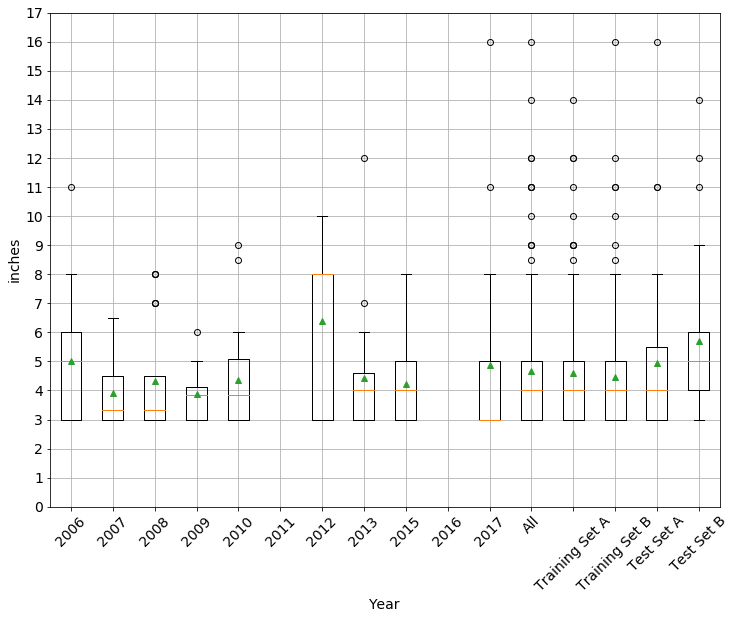
\includegraphics{figs/model_snowfall.png}
\caption{}
\end{figure}

\subsection{Linear Regression
Analysis}\label{linear-regression-analysis}

To assess snowfall prediction potential with Ordinary Least Squares
(OLS) model, a linear regression analysis was performed on each feature
in the dataset. For each potential variable, data was plotted against
snowfall amounts which would occur over the next 12 hours. Slope,
standard error, R square values, along with p values were calculated for
all variables.

A table showing results from this analysis are shown in \textbf{Table
3}. The data are sorted by largest R value. Note that the variables with
the best predictive capabilities are dewpoint, KCCU Wind Speed, and
pressure changes. Though Cloud Cover does have higher R values as well,
the p values and amount of data missing is also very high. While the R
values are not notably high (all are less then 0.2), p values for
dewpoint, 12-hr pressure change are less then 0.05, indicating that
there may be some predictive skill with an OLS model. It is also
important to note that that cloud cover is a categorical variable
(values are in integers from 0 to 8) and wind direction is a circular
variables (values range from 0 to 360 degrees) and do not lend
themselves well to linear regression type statistic. These two variables
should be considered cautiously in a linear regression analysis, but
will be considered in an OLS analysis as some predictive properties may
be

There

\begin{center}\rule{0.5\linewidth}{\linethickness}\end{center}

\textbf{Table 3 - Output statistics from Linear Regression Analysis
{[}1{]}}

\begin{longtable}[]{@{}llllllllllll@{}}
\toprule
\begin{minipage}[b]{0.18\columnwidth}\raggedright\strut
Feature\strut
\end{minipage} & \begin{minipage}[b]{0.04\columnwidth}\raggedright\strut
Max\strut
\end{minipage} & \begin{minipage}[b]{0.04\columnwidth}\raggedright\strut
Min\strut
\end{minipage} & \begin{minipage}[b]{0.04\columnwidth}\raggedright\strut
Mean\strut
\end{minipage} & \begin{minipage}[b]{0.04\columnwidth}\raggedright\strut
Slope\strut
\end{minipage} & \begin{minipage}[b]{0.05\columnwidth}\raggedright\strut
Std Error\strut
\end{minipage} & \begin{minipage}[b]{0.04\columnwidth}\raggedright\strut
R Value\strut
\end{minipage} & \begin{minipage}[b]{0.04\columnwidth}\raggedright\strut
P-value\strut
\end{minipage} & \begin{minipage}[b]{0.05\columnwidth}\raggedright\strut
\% Missing\strut
\end{minipage} & \begin{minipage}[b]{0.05\columnwidth}\raggedright\strut
Abs R\strut
\end{minipage} & \begin{minipage}[b]{0.05\columnwidth}\raggedright\strut
SNF Counts\strut
\end{minipage} & \begin{minipage}[b]{0.07\columnwidth}\raggedright\strut
Feature Counts\strut
\end{minipage}\tabularnewline
\midrule
\endhead
\begin{minipage}[t]{0.18\columnwidth}\raggedright\strut
CMtn\_ CMtn\_Dewpoint\_degC\strut
\end{minipage} & \begin{minipage}[t]{0.04\columnwidth}\raggedright\strut
0.0\strut
\end{minipage} & \begin{minipage}[t]{0.04\columnwidth}\raggedright\strut
-27.0\strut
\end{minipage} & \begin{minipage}[t]{0.04\columnwidth}\raggedright\strut
-9.7\strut
\end{minipage} & \begin{minipage}[t]{0.04\columnwidth}\raggedright\strut
0.081\strut
\end{minipage} & \begin{minipage}[t]{0.05\columnwidth}\raggedright\strut
0.029\strut
\end{minipage} & \begin{minipage}[t]{0.04\columnwidth}\raggedright\strut
0.181\strut
\end{minipage} & \begin{minipage}[t]{0.04\columnwidth}\raggedright\strut
0.006\strut
\end{minipage} & \begin{minipage}[t]{0.05\columnwidth}\raggedright\strut
25.0\strut
\end{minipage} & \begin{minipage}[t]{0.05\columnwidth}\raggedright\strut
0.180794\strut
\end{minipage} & \begin{minipage}[t]{0.05\columnwidth}\raggedright\strut
301\strut
\end{minipage} & \begin{minipage}[t]{0.07\columnwidth}\raggedright\strut
227\strut
\end{minipage}\tabularnewline
\begin{minipage}[t]{0.18\columnwidth}\raggedright\strut
LXV LXV\_Dewpoint\_degC\strut
\end{minipage} & \begin{minipage}[t]{0.04\columnwidth}\raggedright\strut
2.8\strut
\end{minipage} & \begin{minipage}[t]{0.04\columnwidth}\raggedright\strut
-22.8\strut
\end{minipage} & \begin{minipage}[t]{0.04\columnwidth}\raggedright\strut
-8.0\strut
\end{minipage} & \begin{minipage}[t]{0.04\columnwidth}\raggedright\strut
0.083\strut
\end{minipage} & \begin{minipage}[t]{0.05\columnwidth}\raggedright\strut
0.032\strut
\end{minipage} & \begin{minipage}[t]{0.04\columnwidth}\raggedright\strut
0.159\strut
\end{minipage} & \begin{minipage}[t]{0.04\columnwidth}\raggedright\strut
0.009\strut
\end{minipage} & \begin{minipage}[t]{0.05\columnwidth}\raggedright\strut
11.0\strut
\end{minipage} & \begin{minipage}[t]{0.05\columnwidth}\raggedright\strut
0.158541\strut
\end{minipage} & \begin{minipage}[t]{0.05\columnwidth}\raggedright\strut
301\strut
\end{minipage} & \begin{minipage}[t]{0.07\columnwidth}\raggedright\strut
269\strut
\end{minipage}\tabularnewline
\begin{minipage}[t]{0.18\columnwidth}\raggedright\strut
CMtn\_ CMtn\_CloudCover\_oktas\strut
\end{minipage} & \begin{minipage}[t]{0.04\columnwidth}\raggedright\strut
8.0\strut
\end{minipage} & \begin{minipage}[t]{0.04\columnwidth}\raggedright\strut
0.0\strut
\end{minipage} & \begin{minipage}[t]{0.04\columnwidth}\raggedright\strut
7.4\strut
\end{minipage} & \begin{minipage}[t]{0.04\columnwidth}\raggedright\strut
0.145\strut
\end{minipage} & \begin{minipage}[t]{0.05\columnwidth}\raggedright\strut
0.085\strut
\end{minipage} & \begin{minipage}[t]{0.04\columnwidth}\raggedright\strut
0.142\strut
\end{minipage} & \begin{minipage}[t]{0.04\columnwidth}\raggedright\strut
0.089\strut
\end{minipage} & \begin{minipage}[t]{0.05\columnwidth}\raggedright\strut
52.0\strut
\end{minipage} & \begin{minipage}[t]{0.05\columnwidth}\raggedright\strut
0.141753\strut
\end{minipage} & \begin{minipage}[t]{0.05\columnwidth}\raggedright\strut
301\strut
\end{minipage} & \begin{minipage}[t]{0.07\columnwidth}\raggedright\strut
145\strut
\end{minipage}\tabularnewline
\begin{minipage}[t]{0.18\columnwidth}\raggedright\strut
LXV LXV\_CloudCover\_oktas\strut
\end{minipage} & \begin{minipage}[t]{0.04\columnwidth}\raggedright\strut
8.0\strut
\end{minipage} & \begin{minipage}[t]{0.04\columnwidth}\raggedright\strut
0.0\strut
\end{minipage} & \begin{minipage}[t]{0.04\columnwidth}\raggedright\strut
6.8\strut
\end{minipage} & \begin{minipage}[t]{0.04\columnwidth}\raggedright\strut
0.088\strut
\end{minipage} & \begin{minipage}[t]{0.05\columnwidth}\raggedright\strut
0.059\strut
\end{minipage} & \begin{minipage}[t]{0.04\columnwidth}\raggedright\strut
0.122\strut
\end{minipage} & \begin{minipage}[t]{0.04\columnwidth}\raggedright\strut
0.136\strut
\end{minipage} & \begin{minipage}[t]{0.05\columnwidth}\raggedright\strut
50.0\strut
\end{minipage} & \begin{minipage}[t]{0.05\columnwidth}\raggedright\strut
0.121625\strut
\end{minipage} & \begin{minipage}[t]{0.05\columnwidth}\raggedright\strut
301\strut
\end{minipage} & \begin{minipage}[t]{0.07\columnwidth}\raggedright\strut
152\strut
\end{minipage}\tabularnewline
\begin{minipage}[t]{0.18\columnwidth}\raggedright\strut
LXV LXV\_Temperature\_degC\strut
\end{minipage} & \begin{minipage}[t]{0.04\columnwidth}\raggedright\strut
13.3\strut
\end{minipage} & \begin{minipage}[t]{0.04\columnwidth}\raggedright\strut
-17.2\strut
\end{minipage} & \begin{minipage}[t]{0.04\columnwidth}\raggedright\strut
-2.9\strut
\end{minipage} & \begin{minipage}[t]{0.04\columnwidth}\raggedright\strut
0.043\strut
\end{minipage} & \begin{minipage}[t]{0.05\columnwidth}\raggedright\strut
0.026\strut
\end{minipage} & \begin{minipage}[t]{0.04\columnwidth}\raggedright\strut
0.101\strut
\end{minipage} & \begin{minipage}[t]{0.04\columnwidth}\raggedright\strut
0.100\strut
\end{minipage} & \begin{minipage}[t]{0.05\columnwidth}\raggedright\strut
11.0\strut
\end{minipage} & \begin{minipage}[t]{0.05\columnwidth}\raggedright\strut
0.100527\strut
\end{minipage} & \begin{minipage}[t]{0.05\columnwidth}\raggedright\strut
301\strut
\end{minipage} & \begin{minipage}[t]{0.07\columnwidth}\raggedright\strut
269\strut
\end{minipage}\tabularnewline
\begin{minipage}[t]{0.18\columnwidth}\raggedright\strut
LXV LXV\_WindDirection\_deg\strut
\end{minipage} & \begin{minipage}[t]{0.04\columnwidth}\raggedright\strut
360.0\strut
\end{minipage} & \begin{minipage}[t]{0.04\columnwidth}\raggedright\strut
0.0\strut
\end{minipage} & \begin{minipage}[t]{0.04\columnwidth}\raggedright\strut
179.7\strut
\end{minipage} & \begin{minipage}[t]{0.04\columnwidth}\raggedright\strut
-0.002\strut
\end{minipage} & \begin{minipage}[t]{0.05\columnwidth}\raggedright\strut
0.001\strut
\end{minipage} & \begin{minipage}[t]{0.04\columnwidth}\raggedright\strut
-0.098\strut
\end{minipage} & \begin{minipage}[t]{0.04\columnwidth}\raggedright\strut
0.107\strut
\end{minipage} & \begin{minipage}[t]{0.05\columnwidth}\raggedright\strut
11.0\strut
\end{minipage} & \begin{minipage}[t]{0.05\columnwidth}\raggedright\strut
0.098491\strut
\end{minipage} & \begin{minipage}[t]{0.05\columnwidth}\raggedright\strut
301\strut
\end{minipage} & \begin{minipage}[t]{0.07\columnwidth}\raggedright\strut
269\strut
\end{minipage}\tabularnewline
\begin{minipage}[t]{0.18\columnwidth}\raggedright\strut
LXV LXV\_12hr\_delta\_Pressure\_hp\strut
\end{minipage} & \begin{minipage}[t]{0.04\columnwidth}\raggedright\strut
13.3\strut
\end{minipage} & \begin{minipage}[t]{0.04\columnwidth}\raggedright\strut
-20.2\strut
\end{minipage} & \begin{minipage}[t]{0.04\columnwidth}\raggedright\strut
-3.0\strut
\end{minipage} & \begin{minipage}[t]{0.04\columnwidth}\raggedright\strut
-0.039\strut
\end{minipage} & \begin{minipage}[t]{0.05\columnwidth}\raggedright\strut
0.024\strut
\end{minipage} & \begin{minipage}[t]{0.04\columnwidth}\raggedright\strut
-0.098\strut
\end{minipage} & \begin{minipage}[t]{0.04\columnwidth}\raggedright\strut
0.112\strut
\end{minipage} & \begin{minipage}[t]{0.05\columnwidth}\raggedright\strut
12.0\strut
\end{minipage} & \begin{minipage}[t]{0.05\columnwidth}\raggedright\strut
0.0975685\strut
\end{minipage} & \begin{minipage}[t]{0.05\columnwidth}\raggedright\strut
301\strut
\end{minipage} & \begin{minipage}[t]{0.07\columnwidth}\raggedright\strut
266\strut
\end{minipage}\tabularnewline
\begin{minipage}[t]{0.18\columnwidth}\raggedright\strut
CMtnSNTL\_ CMtnSNTL\_Temp\_degC\strut
\end{minipage} & \begin{minipage}[t]{0.04\columnwidth}\raggedright\strut
7.6\strut
\end{minipage} & \begin{minipage}[t]{0.04\columnwidth}\raggedright\strut
-18.7\strut
\end{minipage} & \begin{minipage}[t]{0.04\columnwidth}\raggedright\strut
-3.5\strut
\end{minipage} & \begin{minipage}[t]{0.04\columnwidth}\raggedright\strut
0.050\strut
\end{minipage} & \begin{minipage}[t]{0.05\columnwidth}\raggedright\strut
0.030\strut
\end{minipage} & \begin{minipage}[t]{0.04\columnwidth}\raggedright\strut
0.096\strut
\end{minipage} & \begin{minipage}[t]{0.04\columnwidth}\raggedright\strut
0.098\strut
\end{minipage} & \begin{minipage}[t]{0.05\columnwidth}\raggedright\strut
0.0\strut
\end{minipage} & \begin{minipage}[t]{0.05\columnwidth}\raggedright\strut
0.0955384\strut
\end{minipage} & \begin{minipage}[t]{0.05\columnwidth}\raggedright\strut
301\strut
\end{minipage} & \begin{minipage}[t]{0.07\columnwidth}\raggedright\strut
301\strut
\end{minipage}\tabularnewline
\begin{minipage}[t]{0.18\columnwidth}\raggedright\strut
CMtn\_ CMtn\_Temperature\_degC\strut
\end{minipage} & \begin{minipage}[t]{0.04\columnwidth}\raggedright\strut
7.0\strut
\end{minipage} & \begin{minipage}[t]{0.04\columnwidth}\raggedright\strut
-21.0\strut
\end{minipage} & \begin{minipage}[t]{0.04\columnwidth}\raggedright\strut
-4.7\strut
\end{minipage} & \begin{minipage}[t]{0.04\columnwidth}\raggedright\strut
0.043\strut
\end{minipage} & \begin{minipage}[t]{0.05\columnwidth}\raggedright\strut
0.031\strut
\end{minipage} & \begin{minipage}[t]{0.04\columnwidth}\raggedright\strut
0.092\strut
\end{minipage} & \begin{minipage}[t]{0.04\columnwidth}\raggedright\strut
0.167\strut
\end{minipage} & \begin{minipage}[t]{0.05\columnwidth}\raggedright\strut
25.0\strut
\end{minipage} & \begin{minipage}[t]{0.05\columnwidth}\raggedright\strut
0.0919552\strut
\end{minipage} & \begin{minipage}[t]{0.05\columnwidth}\raggedright\strut
301\strut
\end{minipage} & \begin{minipage}[t]{0.07\columnwidth}\raggedright\strut
227\strut
\end{minipage}\tabularnewline
\begin{minipage}[t]{0.18\columnwidth}\raggedright\strut
CMtn\_ CMtn\_WindDirection\_deg\strut
\end{minipage} & \begin{minipage}[t]{0.04\columnwidth}\raggedright\strut
360.0\strut
\end{minipage} & \begin{minipage}[t]{0.04\columnwidth}\raggedright\strut
0.0\strut
\end{minipage} & \begin{minipage}[t]{0.04\columnwidth}\raggedright\strut
236.0\strut
\end{minipage} & \begin{minipage}[t]{0.04\columnwidth}\raggedright\strut
0.002\strut
\end{minipage} & \begin{minipage}[t]{0.05\columnwidth}\raggedright\strut
0.002\strut
\end{minipage} & \begin{minipage}[t]{0.04\columnwidth}\raggedright\strut
0.072\strut
\end{minipage} & \begin{minipage}[t]{0.04\columnwidth}\raggedright\strut
0.286\strut
\end{minipage} & \begin{minipage}[t]{0.05\columnwidth}\raggedright\strut
27.0\strut
\end{minipage} & \begin{minipage}[t]{0.05\columnwidth}\raggedright\strut
0.0724723\strut
\end{minipage} & \begin{minipage}[t]{0.05\columnwidth}\raggedright\strut
301\strut
\end{minipage} & \begin{minipage}[t]{0.07\columnwidth}\raggedright\strut
219\strut
\end{minipage}\tabularnewline
\begin{minipage}[t]{0.18\columnwidth}\raggedright\strut
CMtn\_ CMtn\_WindSpeed\_mps\strut
\end{minipage} & \begin{minipage}[t]{0.04\columnwidth}\raggedright\strut
16.9\strut
\end{minipage} & \begin{minipage}[t]{0.04\columnwidth}\raggedright\strut
0.0\strut
\end{minipage} & \begin{minipage}[t]{0.04\columnwidth}\raggedright\strut
7.4\strut
\end{minipage} & \begin{minipage}[t]{0.04\columnwidth}\raggedright\strut
0.036\strut
\end{minipage} & \begin{minipage}[t]{0.05\columnwidth}\raggedright\strut
0.036\strut
\end{minipage} & \begin{minipage}[t]{0.04\columnwidth}\raggedright\strut
0.067\strut
\end{minipage} & \begin{minipage}[t]{0.04\columnwidth}\raggedright\strut
0.322\strut
\end{minipage} & \begin{minipage}[t]{0.05\columnwidth}\raggedright\strut
27.0\strut
\end{minipage} & \begin{minipage}[t]{0.05\columnwidth}\raggedright\strut
0.0671684\strut
\end{minipage} & \begin{minipage}[t]{0.05\columnwidth}\raggedright\strut
301\strut
\end{minipage} & \begin{minipage}[t]{0.07\columnwidth}\raggedright\strut
219\strut
\end{minipage}\tabularnewline
\begin{minipage}[t]{0.18\columnwidth}\raggedright\strut
LXV LXV\_6hr\_Precipitation\_mm\strut
\end{minipage} & \begin{minipage}[t]{0.04\columnwidth}\raggedright\strut
10.2\strut
\end{minipage} & \begin{minipage}[t]{0.04\columnwidth}\raggedright\strut
-0.1\strut
\end{minipage} & \begin{minipage}[t]{0.04\columnwidth}\raggedright\strut
0.9\strut
\end{minipage} & \begin{minipage}[t]{0.04\columnwidth}\raggedright\strut
0.088\strut
\end{minipage} & \begin{minipage}[t]{0.05\columnwidth}\raggedright\strut
0.089\strut
\end{minipage} & \begin{minipage}[t]{0.04\columnwidth}\raggedright\strut
0.063\strut
\end{minipage} & \begin{minipage}[t]{0.04\columnwidth}\raggedright\strut
0.325\strut
\end{minipage} & \begin{minipage}[t]{0.05\columnwidth}\raggedright\strut
19.0\strut
\end{minipage} & \begin{minipage}[t]{0.05\columnwidth}\raggedright\strut
0.0633812\strut
\end{minipage} & \begin{minipage}[t]{0.05\columnwidth}\raggedright\strut
301\strut
\end{minipage} & \begin{minipage}[t]{0.07\columnwidth}\raggedright\strut
243\strut
\end{minipage}\tabularnewline
\begin{minipage}[t]{0.18\columnwidth}\raggedright\strut
LXV LXV\_WindSpeed\_mps\strut
\end{minipage} & \begin{minipage}[t]{0.04\columnwidth}\raggedright\strut
11.8\strut
\end{minipage} & \begin{minipage}[t]{0.04\columnwidth}\raggedright\strut
0.0\strut
\end{minipage} & \begin{minipage}[t]{0.04\columnwidth}\raggedright\strut
3.6\strut
\end{minipage} & \begin{minipage}[t]{0.04\columnwidth}\raggedright\strut
-0.047\strut
\end{minipage} & \begin{minipage}[t]{0.05\columnwidth}\raggedright\strut
0.057\strut
\end{minipage} & \begin{minipage}[t]{0.04\columnwidth}\raggedright\strut
-0.051\strut
\end{minipage} & \begin{minipage}[t]{0.04\columnwidth}\raggedright\strut
0.403\strut
\end{minipage} & \begin{minipage}[t]{0.05\columnwidth}\raggedright\strut
11.0\strut
\end{minipage} & \begin{minipage}[t]{0.05\columnwidth}\raggedright\strut
0.051206\strut
\end{minipage} & \begin{minipage}[t]{0.05\columnwidth}\raggedright\strut
301\strut
\end{minipage} & \begin{minipage}[t]{0.07\columnwidth}\raggedright\strut
269\strut
\end{minipage}\tabularnewline
\begin{minipage}[t]{0.18\columnwidth}\raggedright\strut
LXV LXV\_Pressure\_hp\strut
\end{minipage} & \begin{minipage}[t]{0.04\columnwidth}\raggedright\strut
1028.5\strut
\end{minipage} & \begin{minipage}[t]{0.04\columnwidth}\raggedright\strut
983.3\strut
\end{minipage} & \begin{minipage}[t]{0.04\columnwidth}\raggedright\strut
1005.3\strut
\end{minipage} & \begin{minipage}[t]{0.04\columnwidth}\raggedright\strut
-0.013\strut
\end{minipage} & \begin{minipage}[t]{0.05\columnwidth}\raggedright\strut
0.016\strut
\end{minipage} & \begin{minipage}[t]{0.04\columnwidth}\raggedright\strut
-0.050\strut
\end{minipage} & \begin{minipage}[t]{0.04\columnwidth}\raggedright\strut
0.420\strut
\end{minipage} & \begin{minipage}[t]{0.05\columnwidth}\raggedright\strut
11.0\strut
\end{minipage} & \begin{minipage}[t]{0.05\columnwidth}\raggedright\strut
0.0495101\strut
\end{minipage} & \begin{minipage}[t]{0.05\columnwidth}\raggedright\strut
301\strut
\end{minipage} & \begin{minipage}[t]{0.07\columnwidth}\raggedright\strut
267\strut
\end{minipage}\tabularnewline
\bottomrule
\end{longtable}

{[}1{]} Feature statistics are calculated based on only 12-hr values
which have a matching 12-hr snowfall value

\begin{longtable}[]{@{}llllllllllll@{}}
\toprule
\begin{minipage}[b]{0.18\columnwidth}\raggedright\strut
Feature\strut
\end{minipage} & \begin{minipage}[b]{0.04\columnwidth}\raggedright\strut
Max\strut
\end{minipage} & \begin{minipage}[b]{0.04\columnwidth}\raggedright\strut
Min\strut
\end{minipage} & \begin{minipage}[b]{0.04\columnwidth}\raggedright\strut
Mean\strut
\end{minipage} & \begin{minipage}[b]{0.04\columnwidth}\raggedright\strut
Slope\strut
\end{minipage} & \begin{minipage}[b]{0.05\columnwidth}\raggedright\strut
Std Error\strut
\end{minipage} & \begin{minipage}[b]{0.04\columnwidth}\raggedright\strut
R Value\strut
\end{minipage} & \begin{minipage}[b]{0.04\columnwidth}\raggedright\strut
P-value\strut
\end{minipage} & \begin{minipage}[b]{0.05\columnwidth}\raggedright\strut
\% Missing\strut
\end{minipage} & \begin{minipage}[b]{0.05\columnwidth}\raggedright\strut
Abs R\strut
\end{minipage} & \begin{minipage}[b]{0.05\columnwidth}\raggedright\strut
SNF Counts\strut
\end{minipage} & \begin{minipage}[b]{0.07\columnwidth}\raggedright\strut
Feature Counts\strut
\end{minipage}\tabularnewline
\midrule
\endhead
\begin{minipage}[t]{0.18\columnwidth}\raggedright\strut
CMtn\_ CMtn\_Dewpoint\_degC\strut
\end{minipage} & \begin{minipage}[t]{0.04\columnwidth}\raggedright\strut
0.0\strut
\end{minipage} & \begin{minipage}[t]{0.04\columnwidth}\raggedright\strut
-27.0\strut
\end{minipage} & \begin{minipage}[t]{0.04\columnwidth}\raggedright\strut
-9.7\strut
\end{minipage} & \begin{minipage}[t]{0.04\columnwidth}\raggedright\strut
0.081\strut
\end{minipage} & \begin{minipage}[t]{0.05\columnwidth}\raggedright\strut
0.029\strut
\end{minipage} & \begin{minipage}[t]{0.04\columnwidth}\raggedright\strut
0.181\strut
\end{minipage} & \begin{minipage}[t]{0.04\columnwidth}\raggedright\strut
0.006\strut
\end{minipage} & \begin{minipage}[t]{0.05\columnwidth}\raggedright\strut
25.0\strut
\end{minipage} & \begin{minipage}[t]{0.05\columnwidth}\raggedright\strut
0.180794\strut
\end{minipage} & \begin{minipage}[t]{0.05\columnwidth}\raggedright\strut
301\strut
\end{minipage} & \begin{minipage}[t]{0.07\columnwidth}\raggedright\strut
227\strut
\end{minipage}\tabularnewline
\begin{minipage}[t]{0.18\columnwidth}\raggedright\strut
speed\_kts KGJT\_250mb\_speed\_kts\strut
\end{minipage} & \begin{minipage}[t]{0.04\columnwidth}\raggedright\strut
163.0\strut
\end{minipage} & \begin{minipage}[t]{0.04\columnwidth}\raggedright\strut
8.0\strut
\end{minipage} & \begin{minipage}[t]{0.04\columnwidth}\raggedright\strut
76.4\strut
\end{minipage} & \begin{minipage}[t]{0.04\columnwidth}\raggedright\strut
0.011\strut
\end{minipage} & \begin{minipage}[t]{0.05\columnwidth}\raggedright\strut
0.004\strut
\end{minipage} & \begin{minipage}[t]{0.04\columnwidth}\raggedright\strut
0.172\strut
\end{minipage} & \begin{minipage}[t]{0.04\columnwidth}\raggedright\strut
0.003\strut
\end{minipage} & \begin{minipage}[t]{0.05\columnwidth}\raggedright\strut
2.0\strut
\end{minipage} & \begin{minipage}[t]{0.05\columnwidth}\raggedright\strut
0.17217\strut
\end{minipage} & \begin{minipage}[t]{0.05\columnwidth}\raggedright\strut
301\strut
\end{minipage} & \begin{minipage}[t]{0.07\columnwidth}\raggedright\strut
295\strut
\end{minipage}\tabularnewline
\begin{minipage}[t]{0.18\columnwidth}\raggedright\strut
speed\_kts KGJT\_300mb\_speed\_kts\strut
\end{minipage} & \begin{minipage}[t]{0.04\columnwidth}\raggedright\strut
151.0\strut
\end{minipage} & \begin{minipage}[t]{0.04\columnwidth}\raggedright\strut
7.0\strut
\end{minipage} & \begin{minipage}[t]{0.04\columnwidth}\raggedright\strut
71.8\strut
\end{minipage} & \begin{minipage}[t]{0.04\columnwidth}\raggedright\strut
0.012\strut
\end{minipage} & \begin{minipage}[t]{0.05\columnwidth}\raggedright\strut
0.004\strut
\end{minipage} & \begin{minipage}[t]{0.04\columnwidth}\raggedright\strut
0.167\strut
\end{minipage} & \begin{minipage}[t]{0.04\columnwidth}\raggedright\strut
0.004\strut
\end{minipage} & \begin{minipage}[t]{0.05\columnwidth}\raggedright\strut
2.0\strut
\end{minipage} & \begin{minipage}[t]{0.05\columnwidth}\raggedright\strut
0.167416\strut
\end{minipage} & \begin{minipage}[t]{0.05\columnwidth}\raggedright\strut
301\strut
\end{minipage} & \begin{minipage}[t]{0.07\columnwidth}\raggedright\strut
296\strut
\end{minipage}\tabularnewline
\begin{minipage}[t]{0.18\columnwidth}\raggedright\strut
speed\_kts KGJT\_400mb\_speed\_kts\strut
\end{minipage} & \begin{minipage}[t]{0.04\columnwidth}\raggedright\strut
116.0\strut
\end{minipage} & \begin{minipage}[t]{0.04\columnwidth}\raggedright\strut
4.0\strut
\end{minipage} & \begin{minipage}[t]{0.04\columnwidth}\raggedright\strut
54.0\strut
\end{minipage} & \begin{minipage}[t]{0.04\columnwidth}\raggedright\strut
0.015\strut
\end{minipage} & \begin{minipage}[t]{0.05\columnwidth}\raggedright\strut
0.005\strut
\end{minipage} & \begin{minipage}[t]{0.04\columnwidth}\raggedright\strut
0.167\strut
\end{minipage} & \begin{minipage}[t]{0.04\columnwidth}\raggedright\strut
0.004\strut
\end{minipage} & \begin{minipage}[t]{0.05\columnwidth}\raggedright\strut
1.0\strut
\end{minipage} & \begin{minipage}[t]{0.05\columnwidth}\raggedright\strut
0.167206\strut
\end{minipage} & \begin{minipage}[t]{0.05\columnwidth}\raggedright\strut
301\strut
\end{minipage} & \begin{minipage}[t]{0.07\columnwidth}\raggedright\strut
299\strut
\end{minipage}\tabularnewline
\begin{minipage}[t]{0.18\columnwidth}\raggedright\strut
height\_m KGJT\_d500\_400\_height\_m\strut
\end{minipage} & \begin{minipage}[t]{0.04\columnwidth}\raggedright\strut
-1550.0\strut
\end{minipage} & \begin{minipage}[t]{0.04\columnwidth}\raggedright\strut
-1680.0\strut
\end{minipage} & \begin{minipage}[t]{0.04\columnwidth}\raggedright\strut
-1613.1\strut
\end{minipage} & \begin{minipage}[t]{0.04\columnwidth}\raggedright\strut
-0.014\strut
\end{minipage} & \begin{minipage}[t]{0.05\columnwidth}\raggedright\strut
0.005\strut
\end{minipage} & \begin{minipage}[t]{0.04\columnwidth}\raggedright\strut
-0.166\strut
\end{minipage} & \begin{minipage}[t]{0.04\columnwidth}\raggedright\strut
0.004\strut
\end{minipage} & \begin{minipage}[t]{0.05\columnwidth}\raggedright\strut
1.0\strut
\end{minipage} & \begin{minipage}[t]{0.05\columnwidth}\raggedright\strut
0.166312\strut
\end{minipage} & \begin{minipage}[t]{0.05\columnwidth}\raggedright\strut
301\strut
\end{minipage} & \begin{minipage}[t]{0.07\columnwidth}\raggedright\strut
299\strut
\end{minipage}\tabularnewline
\begin{minipage}[t]{0.18\columnwidth}\raggedright\strut
tmpc KGJT\_400mb\_tmpc\strut
\end{minipage} & \begin{minipage}[t]{0.04\columnwidth}\raggedright\strut
-22.7\strut
\end{minipage} & \begin{minipage}[t]{0.04\columnwidth}\raggedright\strut
-42.5\strut
\end{minipage} & \begin{minipage}[t]{0.04\columnwidth}\raggedright\strut
-32.3\strut
\end{minipage} & \begin{minipage}[t]{0.04\columnwidth}\raggedright\strut
0.087\strut
\end{minipage} & \begin{minipage}[t]{0.05\columnwidth}\raggedright\strut
0.031\strut
\end{minipage} & \begin{minipage}[t]{0.04\columnwidth}\raggedright\strut
0.162\strut
\end{minipage} & \begin{minipage}[t]{0.04\columnwidth}\raggedright\strut
0.005\strut
\end{minipage} & \begin{minipage}[t]{0.05\columnwidth}\raggedright\strut
1.0\strut
\end{minipage} & \begin{minipage}[t]{0.05\columnwidth}\raggedright\strut
0.161833\strut
\end{minipage} & \begin{minipage}[t]{0.05\columnwidth}\raggedright\strut
301\strut
\end{minipage} & \begin{minipage}[t]{0.07\columnwidth}\raggedright\strut
299\strut
\end{minipage}\tabularnewline
\begin{minipage}[t]{0.18\columnwidth}\raggedright\strut
LXV LXV\_Dewpoint\_degC\strut
\end{minipage} & \begin{minipage}[t]{0.04\columnwidth}\raggedright\strut
2.8\strut
\end{minipage} & \begin{minipage}[t]{0.04\columnwidth}\raggedright\strut
-22.8\strut
\end{minipage} & \begin{minipage}[t]{0.04\columnwidth}\raggedright\strut
-8.0\strut
\end{minipage} & \begin{minipage}[t]{0.04\columnwidth}\raggedright\strut
0.083\strut
\end{minipage} & \begin{minipage}[t]{0.05\columnwidth}\raggedright\strut
0.032\strut
\end{minipage} & \begin{minipage}[t]{0.04\columnwidth}\raggedright\strut
0.159\strut
\end{minipage} & \begin{minipage}[t]{0.04\columnwidth}\raggedright\strut
0.009\strut
\end{minipage} & \begin{minipage}[t]{0.05\columnwidth}\raggedright\strut
11.0\strut
\end{minipage} & \begin{minipage}[t]{0.05\columnwidth}\raggedright\strut
0.158541\strut
\end{minipage} & \begin{minipage}[t]{0.05\columnwidth}\raggedright\strut
301\strut
\end{minipage} & \begin{minipage}[t]{0.07\columnwidth}\raggedright\strut
269\strut
\end{minipage}\tabularnewline
\begin{minipage}[t]{0.18\columnwidth}\raggedright\strut
speed\_kts KGJT\_500mb\_speed\_kts\strut
\end{minipage} & \begin{minipage}[t]{0.04\columnwidth}\raggedright\strut
96.0\strut
\end{minipage} & \begin{minipage}[t]{0.04\columnwidth}\raggedright\strut
2.0\strut
\end{minipage} & \begin{minipage}[t]{0.04\columnwidth}\raggedright\strut
41.4\strut
\end{minipage} & \begin{minipage}[t]{0.04\columnwidth}\raggedright\strut
0.018\strut
\end{minipage} & \begin{minipage}[t]{0.05\columnwidth}\raggedright\strut
0.007\strut
\end{minipage} & \begin{minipage}[t]{0.04\columnwidth}\raggedright\strut
0.153\strut
\end{minipage} & \begin{minipage}[t]{0.04\columnwidth}\raggedright\strut
0.008\strut
\end{minipage} & \begin{minipage}[t]{0.05\columnwidth}\raggedright\strut
1.0\strut
\end{minipage} & \begin{minipage}[t]{0.05\columnwidth}\raggedright\strut
0.153061\strut
\end{minipage} & \begin{minipage}[t]{0.05\columnwidth}\raggedright\strut
301\strut
\end{minipage} & \begin{minipage}[t]{0.07\columnwidth}\raggedright\strut
299\strut
\end{minipage}\tabularnewline
\begin{minipage}[t]{0.18\columnwidth}\raggedright\strut
height\_m KGJT\_d500\_300\_height\_m\strut
\end{minipage} & \begin{minipage}[t]{0.04\columnwidth}\raggedright\strut
-3470.0\strut
\end{minipage} & \begin{minipage}[t]{0.04\columnwidth}\raggedright\strut
-3710.0\strut
\end{minipage} & \begin{minipage}[t]{0.04\columnwidth}\raggedright\strut
-3580.0\strut
\end{minipage} & \begin{minipage}[t]{0.04\columnwidth}\raggedright\strut
-0.006\strut
\end{minipage} & \begin{minipage}[t]{0.05\columnwidth}\raggedright\strut
0.002\strut
\end{minipage} & \begin{minipage}[t]{0.04\columnwidth}\raggedright\strut
-0.153\strut
\end{minipage} & \begin{minipage}[t]{0.04\columnwidth}\raggedright\strut
0.008\strut
\end{minipage} & \begin{minipage}[t]{0.05\columnwidth}\raggedright\strut
1.0\strut
\end{minipage} & \begin{minipage}[t]{0.05\columnwidth}\raggedright\strut
0.152943\strut
\end{minipage} & \begin{minipage}[t]{0.05\columnwidth}\raggedright\strut
301\strut
\end{minipage} & \begin{minipage}[t]{0.07\columnwidth}\raggedright\strut
299\strut
\end{minipage}\tabularnewline
\begin{minipage}[t]{0.18\columnwidth}\raggedright\strut
speed\_kts KGJT\_d700\_250\_speed\_kts\strut
\end{minipage} & \begin{minipage}[t]{0.04\columnwidth}\raggedright\strut
12.0\strut
\end{minipage} & \begin{minipage}[t]{0.04\columnwidth}\raggedright\strut
-132.0\strut
\end{minipage} & \begin{minipage}[t]{0.04\columnwidth}\raggedright\strut
-55.3\strut
\end{minipage} & \begin{minipage}[t]{0.04\columnwidth}\raggedright\strut
-0.011\strut
\end{minipage} & \begin{minipage}[t]{0.05\columnwidth}\raggedright\strut
0.004\strut
\end{minipage} & \begin{minipage}[t]{0.04\columnwidth}\raggedright\strut
-0.152\strut
\end{minipage} & \begin{minipage}[t]{0.04\columnwidth}\raggedright\strut
0.009\strut
\end{minipage} & \begin{minipage}[t]{0.05\columnwidth}\raggedright\strut
2.0\strut
\end{minipage} & \begin{minipage}[t]{0.05\columnwidth}\raggedright\strut
0.152038\strut
\end{minipage} & \begin{minipage}[t]{0.05\columnwidth}\raggedright\strut
301\strut
\end{minipage} & \begin{minipage}[t]{0.07\columnwidth}\raggedright\strut
295\strut
\end{minipage}\tabularnewline
\begin{minipage}[t]{0.18\columnwidth}\raggedright\strut
drct KGJT\_d700\_500\_drct\strut
\end{minipage} & \begin{minipage}[t]{0.04\columnwidth}\raggedright\strut
345.0\strut
\end{minipage} & \begin{minipage}[t]{0.04\columnwidth}\raggedright\strut
-355.0\strut
\end{minipage} & \begin{minipage}[t]{0.04\columnwidth}\raggedright\strut
-8.4\strut
\end{minipage} & \begin{minipage}[t]{0.04\columnwidth}\raggedright\strut
0.004\strut
\end{minipage} & \begin{minipage}[t]{0.05\columnwidth}\raggedright\strut
0.002\strut
\end{minipage} & \begin{minipage}[t]{0.04\columnwidth}\raggedright\strut
0.151\strut
\end{minipage} & \begin{minipage}[t]{0.04\columnwidth}\raggedright\strut
0.009\strut
\end{minipage} & \begin{minipage}[t]{0.05\columnwidth}\raggedright\strut
1.0\strut
\end{minipage} & \begin{minipage}[t]{0.05\columnwidth}\raggedright\strut
0.150643\strut
\end{minipage} & \begin{minipage}[t]{0.05\columnwidth}\raggedright\strut
301\strut
\end{minipage} & \begin{minipage}[t]{0.07\columnwidth}\raggedright\strut
299\strut
\end{minipage}\tabularnewline
\begin{minipage}[t]{0.18\columnwidth}\raggedright\strut
tmpc KGJT\_500mb\_tmpc\strut
\end{minipage} & \begin{minipage}[t]{0.04\columnwidth}\raggedright\strut
-9.9\strut
\end{minipage} & \begin{minipage}[t]{0.04\columnwidth}\raggedright\strut
-30.5\strut
\end{minipage} & \begin{minipage}[t]{0.04\columnwidth}\raggedright\strut
-20.4\strut
\end{minipage} & \begin{minipage}[t]{0.04\columnwidth}\raggedright\strut
0.084\strut
\end{minipage} & \begin{minipage}[t]{0.05\columnwidth}\raggedright\strut
0.033\strut
\end{minipage} & \begin{minipage}[t]{0.04\columnwidth}\raggedright\strut
0.145\strut
\end{minipage} & \begin{minipage}[t]{0.04\columnwidth}\raggedright\strut
0.012\strut
\end{minipage} & \begin{minipage}[t]{0.05\columnwidth}\raggedright\strut
1.0\strut
\end{minipage} & \begin{minipage}[t]{0.05\columnwidth}\raggedright\strut
0.145121\strut
\end{minipage} & \begin{minipage}[t]{0.05\columnwidth}\raggedright\strut
301\strut
\end{minipage} & \begin{minipage}[t]{0.07\columnwidth}\raggedright\strut
299\strut
\end{minipage}\tabularnewline
\begin{minipage}[t]{0.18\columnwidth}\raggedright\strut
height\_m KGJT\_d700\_300\_height\_m\strut
\end{minipage} & \begin{minipage}[t]{0.04\columnwidth}\raggedright\strut
-5979.0\strut
\end{minipage} & \begin{minipage}[t]{0.04\columnwidth}\raggedright\strut
-6391.0\strut
\end{minipage} & \begin{minipage}[t]{0.04\columnwidth}\raggedright\strut
-6156.1\strut
\end{minipage} & \begin{minipage}[t]{0.04\columnwidth}\raggedright\strut
-0.004\strut
\end{minipage} & \begin{minipage}[t]{0.05\columnwidth}\raggedright\strut
0.001\strut
\end{minipage} & \begin{minipage}[t]{0.04\columnwidth}\raggedright\strut
-0.145\strut
\end{minipage} & \begin{minipage}[t]{0.04\columnwidth}\raggedright\strut
0.012\strut
\end{minipage} & \begin{minipage}[t]{0.05\columnwidth}\raggedright\strut
1.0\strut
\end{minipage} & \begin{minipage}[t]{0.05\columnwidth}\raggedright\strut
0.144929\strut
\end{minipage} & \begin{minipage}[t]{0.05\columnwidth}\raggedright\strut
301\strut
\end{minipage} & \begin{minipage}[t]{0.07\columnwidth}\raggedright\strut
299\strut
\end{minipage}\tabularnewline
\begin{minipage}[t]{0.18\columnwidth}\raggedright\strut
speed\_kts KGJT\_d700\_300\_speed\_kts\strut
\end{minipage} & \begin{minipage}[t]{0.04\columnwidth}\raggedright\strut
23.0\strut
\end{minipage} & \begin{minipage}[t]{0.04\columnwidth}\raggedright\strut
-131.0\strut
\end{minipage} & \begin{minipage}[t]{0.04\columnwidth}\raggedright\strut
-50.7\strut
\end{minipage} & \begin{minipage}[t]{0.04\columnwidth}\raggedright\strut
-0.011\strut
\end{minipage} & \begin{minipage}[t]{0.05\columnwidth}\raggedright\strut
0.004\strut
\end{minipage} & \begin{minipage}[t]{0.04\columnwidth}\raggedright\strut
-0.144\strut
\end{minipage} & \begin{minipage}[t]{0.04\columnwidth}\raggedright\strut
0.013\strut
\end{minipage} & \begin{minipage}[t]{0.05\columnwidth}\raggedright\strut
2.0\strut
\end{minipage} & \begin{minipage}[t]{0.05\columnwidth}\raggedright\strut
0.143623\strut
\end{minipage} & \begin{minipage}[t]{0.05\columnwidth}\raggedright\strut
301\strut
\end{minipage} & \begin{minipage}[t]{0.07\columnwidth}\raggedright\strut
296\strut
\end{minipage}\tabularnewline
\begin{minipage}[t]{0.18\columnwidth}\raggedright\strut
height\_m KGJT\_d500\_250\_height\_m\strut
\end{minipage} & \begin{minipage}[t]{0.04\columnwidth}\raggedright\strut
-4620.0\strut
\end{minipage} & \begin{minipage}[t]{0.04\columnwidth}\raggedright\strut
-4970.0\strut
\end{minipage} & \begin{minipage}[t]{0.04\columnwidth}\raggedright\strut
-4772.4\strut
\end{minipage} & \begin{minipage}[t]{0.04\columnwidth}\raggedright\strut
-0.005\strut
\end{minipage} & \begin{minipage}[t]{0.05\columnwidth}\raggedright\strut
0.002\strut
\end{minipage} & \begin{minipage}[t]{0.04\columnwidth}\raggedright\strut
-0.142\strut
\end{minipage} & \begin{minipage}[t]{0.04\columnwidth}\raggedright\strut
0.014\strut
\end{minipage} & \begin{minipage}[t]{0.05\columnwidth}\raggedright\strut
1.0\strut
\end{minipage} & \begin{minipage}[t]{0.05\columnwidth}\raggedright\strut
0.142035\strut
\end{minipage} & \begin{minipage}[t]{0.05\columnwidth}\raggedright\strut
301\strut
\end{minipage} & \begin{minipage}[t]{0.07\columnwidth}\raggedright\strut
299\strut
\end{minipage}\tabularnewline
\begin{minipage}[t]{0.18\columnwidth}\raggedright\strut
height\_m KGJT\_d700\_400\_height\_m\strut
\end{minipage} & \begin{minipage}[t]{0.04\columnwidth}\raggedright\strut
-4055.0\strut
\end{minipage} & \begin{minipage}[t]{0.04\columnwidth}\raggedright\strut
-4361.0\strut
\end{minipage} & \begin{minipage}[t]{0.04\columnwidth}\raggedright\strut
-4189.3\strut
\end{minipage} & \begin{minipage}[t]{0.04\columnwidth}\raggedright\strut
-0.005\strut
\end{minipage} & \begin{minipage}[t]{0.05\columnwidth}\raggedright\strut
0.002\strut
\end{minipage} & \begin{minipage}[t]{0.04\columnwidth}\raggedright\strut
-0.142\strut
\end{minipage} & \begin{minipage}[t]{0.04\columnwidth}\raggedright\strut
0.014\strut
\end{minipage} & \begin{minipage}[t]{0.05\columnwidth}\raggedright\strut
1.0\strut
\end{minipage} & \begin{minipage}[t]{0.05\columnwidth}\raggedright\strut
0.141794\strut
\end{minipage} & \begin{minipage}[t]{0.05\columnwidth}\raggedright\strut
301\strut
\end{minipage} & \begin{minipage}[t]{0.07\columnwidth}\raggedright\strut
299\strut
\end{minipage}\tabularnewline
\begin{minipage}[t]{0.18\columnwidth}\raggedright\strut
speed\_kts KGJT\_200mb\_speed\_kts\strut
\end{minipage} & \begin{minipage}[t]{0.04\columnwidth}\raggedright\strut
157.0\strut
\end{minipage} & \begin{minipage}[t]{0.04\columnwidth}\raggedright\strut
5.0\strut
\end{minipage} & \begin{minipage}[t]{0.04\columnwidth}\raggedright\strut
69.9\strut
\end{minipage} & \begin{minipage}[t]{0.04\columnwidth}\raggedright\strut
0.010\strut
\end{minipage} & \begin{minipage}[t]{0.05\columnwidth}\raggedright\strut
0.004\strut
\end{minipage} & \begin{minipage}[t]{0.04\columnwidth}\raggedright\strut
0.142\strut
\end{minipage} & \begin{minipage}[t]{0.04\columnwidth}\raggedright\strut
0.015\strut
\end{minipage} & \begin{minipage}[t]{0.05\columnwidth}\raggedright\strut
3.0\strut
\end{minipage} & \begin{minipage}[t]{0.05\columnwidth}\raggedright\strut
0.141705\strut
\end{minipage} & \begin{minipage}[t]{0.05\columnwidth}\raggedright\strut
301\strut
\end{minipage} & \begin{minipage}[t]{0.07\columnwidth}\raggedright\strut
292\strut
\end{minipage}\tabularnewline
\begin{minipage}[t]{0.18\columnwidth}\raggedright\strut
height\_m KGJT\_d700\_250\_height\_m\strut
\end{minipage} & \begin{minipage}[t]{0.04\columnwidth}\raggedright\strut
-7139.0\strut
\end{minipage} & \begin{minipage}[t]{0.04\columnwidth}\raggedright\strut
-7611.0\strut
\end{minipage} & \begin{minipage}[t]{0.04\columnwidth}\raggedright\strut
-7348.5\strut
\end{minipage} & \begin{minipage}[t]{0.04\columnwidth}\raggedright\strut
-0.003\strut
\end{minipage} & \begin{minipage}[t]{0.05\columnwidth}\raggedright\strut
0.001\strut
\end{minipage} & \begin{minipage}[t]{0.04\columnwidth}\raggedright\strut
-0.141\strut
\end{minipage} & \begin{minipage}[t]{0.04\columnwidth}\raggedright\strut
0.015\strut
\end{minipage} & \begin{minipage}[t]{0.05\columnwidth}\raggedright\strut
1.0\strut
\end{minipage} & \begin{minipage}[t]{0.05\columnwidth}\raggedright\strut
0.141036\strut
\end{minipage} & \begin{minipage}[t]{0.05\columnwidth}\raggedright\strut
301\strut
\end{minipage} & \begin{minipage}[t]{0.07\columnwidth}\raggedright\strut
299\strut
\end{minipage}\tabularnewline
\begin{minipage}[t]{0.18\columnwidth}\raggedright\strut
drct KGJT\_700mb\_drct\strut
\end{minipage} & \begin{minipage}[t]{0.04\columnwidth}\raggedright\strut
355.0\strut
\end{minipage} & \begin{minipage}[t]{0.04\columnwidth}\raggedright\strut
0.0\strut
\end{minipage} & \begin{minipage}[t]{0.04\columnwidth}\raggedright\strut
247.4\strut
\end{minipage} & \begin{minipage}[t]{0.04\columnwidth}\raggedright\strut
0.005\strut
\end{minipage} & \begin{minipage}[t]{0.05\columnwidth}\raggedright\strut
0.002\strut
\end{minipage} & \begin{minipage}[t]{0.04\columnwidth}\raggedright\strut
0.139\strut
\end{minipage} & \begin{minipage}[t]{0.04\columnwidth}\raggedright\strut
0.016\strut
\end{minipage} & \begin{minipage}[t]{0.05\columnwidth}\raggedright\strut
1.0\strut
\end{minipage} & \begin{minipage}[t]{0.05\columnwidth}\raggedright\strut
0.138809\strut
\end{minipage} & \begin{minipage}[t]{0.05\columnwidth}\raggedright\strut
301\strut
\end{minipage} & \begin{minipage}[t]{0.07\columnwidth}\raggedright\strut
299\strut
\end{minipage}\tabularnewline
\begin{minipage}[t]{0.18\columnwidth}\raggedright\strut
tmpc KGJT\_d700\_400\_tmpc\strut
\end{minipage} & \begin{minipage}[t]{0.04\columnwidth}\raggedright\strut
38.9\strut
\end{minipage} & \begin{minipage}[t]{0.04\columnwidth}\raggedright\strut
16.8\strut
\end{minipage} & \begin{minipage}[t]{0.04\columnwidth}\raggedright\strut
29.3\strut
\end{minipage} & \begin{minipage}[t]{0.04\columnwidth}\raggedright\strut
-0.072\strut
\end{minipage} & \begin{minipage}[t]{0.05\columnwidth}\raggedright\strut
0.030\strut
\end{minipage} & \begin{minipage}[t]{0.04\columnwidth}\raggedright\strut
-0.138\strut
\end{minipage} & \begin{minipage}[t]{0.04\columnwidth}\raggedright\strut
0.017\strut
\end{minipage} & \begin{minipage}[t]{0.05\columnwidth}\raggedright\strut
1.0\strut
\end{minipage} & \begin{minipage}[t]{0.05\columnwidth}\raggedright\strut
0.138276\strut
\end{minipage} & \begin{minipage}[t]{0.05\columnwidth}\raggedright\strut
301\strut
\end{minipage} & \begin{minipage}[t]{0.07\columnwidth}\raggedright\strut
299\strut
\end{minipage}\tabularnewline
\begin{minipage}[t]{0.18\columnwidth}\raggedright\strut
drct KGJT\_d500\_250\_drct\strut
\end{minipage} & \begin{minipage}[t]{0.04\columnwidth}\raggedright\strut
350.0\strut
\end{minipage} & \begin{minipage}[t]{0.04\columnwidth}\raggedright\strut
-85.0\strut
\end{minipage} & \begin{minipage}[t]{0.04\columnwidth}\raggedright\strut
-0.1\strut
\end{minipage} & \begin{minipage}[t]{0.04\columnwidth}\raggedright\strut
-0.006\strut
\end{minipage} & \begin{minipage}[t]{0.05\columnwidth}\raggedright\strut
0.003\strut
\end{minipage} & \begin{minipage}[t]{0.04\columnwidth}\raggedright\strut
-0.133\strut
\end{minipage} & \begin{minipage}[t]{0.04\columnwidth}\raggedright\strut
0.023\strut
\end{minipage} & \begin{minipage}[t]{0.05\columnwidth}\raggedright\strut
2.0\strut
\end{minipage} & \begin{minipage}[t]{0.05\columnwidth}\raggedright\strut
0.13254\strut
\end{minipage} & \begin{minipage}[t]{0.05\columnwidth}\raggedright\strut
301\strut
\end{minipage} & \begin{minipage}[t]{0.07\columnwidth}\raggedright\strut
295\strut
\end{minipage}\tabularnewline
\bottomrule
\end{longtable}

\subsection{OLS Model}\label{ols-model}

Utilizing the statsmodel api with the meteorological datasets, the OLS
function was utilized to determine best fit parameters for a OLS model.
To train the model, years 2006 and 2017 were used as the testing set,
while years (2007-2018) of the meteorological datasets were used as the
traiing set. Two different analyses were performed - one only utilizing
surface meteorological variables, and the other utilizing both upper air
and surface variables. A forward stepwise approach was used using the
adjusted R squared value as the metric to determine the best combination
of coefficient. To perform forward stepwise iternations, model was first
fitted containing a single predictors. Predictors are then added to the
model, one at the time. The adjusted R squared value is calcuated at
each step, and the variable that gave the greatest additional
improvement to the fit is added to the model. At the end of the steps,
the combination of predictors which gave the highest predictive value to
the model will have been found.

\subsubsection{Table 1 - OLS Model Statistics Using Partition
A}\label{table-1---ols-model-statistics-using-partition-a}

\begin{longtable}[]{@{}ccccccccc@{}}
\toprule
\begin{minipage}[b]{0.10\columnwidth}\centering\strut
OLS Model\strut
\end{minipage} & \begin{minipage}[b]{0.04\columnwidth}\centering\strut
R-squared\strut
\end{minipage} & \begin{minipage}[b]{0.06\columnwidth}\centering\strut
Adj. R-squared:\strut
\end{minipage} & \begin{minipage}[b]{0.06\columnwidth}\centering\strut
F-statistic:\strut
\end{minipage} & \begin{minipage}[b]{0.08\columnwidth}\centering\strut
Prob (F-statistic):\strut
\end{minipage} & \begin{minipage}[b]{0.06\columnwidth}\centering\strut
Log-Likelihood:\strut
\end{minipage} & \begin{minipage}[b]{0.03\columnwidth}\centering\strut
AIC:\strut
\end{minipage} & \begin{minipage}[b]{0.03\columnwidth}\centering\strut
BIC:\strut
\end{minipage} & \begin{minipage}[b]{0.30\columnwidth}\centering\strut
Combination of Best Fit Features in OLS\strut
\end{minipage}\tabularnewline
\midrule
\endhead
\begin{minipage}[t]{0.10\columnwidth}\centering\strut
Surface Data Only P1\strut
\end{minipage} & \begin{minipage}[t]{0.04\columnwidth}\centering\strut
0.060\strut
\end{minipage} & \begin{minipage}[t]{0.06\columnwidth}\centering\strut
0.044\strut
\end{minipage} & \begin{minipage}[t]{0.06\columnwidth}\centering\strut
3.765\strut
\end{minipage} & \begin{minipage}[t]{0.08\columnwidth}\centering\strut
0.0118\strut
\end{minipage} & \begin{minipage}[t]{0.06\columnwidth}\centering\strut
-371.85\strut
\end{minipage} & \begin{minipage}[t]{0.03\columnwidth}\centering\strut
751.7\strut
\end{minipage} & \begin{minipage}[t]{0.03\columnwidth}\centering\strut
1019\strut
\end{minipage} & \begin{minipage}[t]{0.30\columnwidth}\centering\strut
LXV\_12hr\_delta\_Pressure\_hp, CMtn\_Dewpoint\_degC,
CMtn\_WindSpeed\_mps\strut
\end{minipage}\tabularnewline
\begin{minipage}[t]{0.10\columnwidth}\centering\strut
Surface+Upper Air Data P1\strut
\end{minipage} & \begin{minipage}[t]{0.04\columnwidth}\centering\strut
0.191\strut
\end{minipage} & \begin{minipage}[t]{0.06\columnwidth}\centering\strut
0.129\strut
\end{minipage} & \begin{minipage}[t]{0.06\columnwidth}\centering\strut
3.087\strut
\end{minipage} & \begin{minipage}[t]{0.08\columnwidth}\centering\strut
0.000606\strut
\end{minipage} & \begin{minipage}[t]{0.06\columnwidth}\centering\strut
-341.66\strut
\end{minipage} & \begin{minipage}[t]{0.03\columnwidth}\centering\strut
709.3\strut
\end{minipage} & \begin{minipage}[t]{0.03\columnwidth}\centering\strut
750.1\strut
\end{minipage} & \begin{minipage}[t]{0.30\columnwidth}\centering\strut
KGJT\_d400\_250\_dwpc, CMtnSNTL\_Temp\_degC,
LXV\_12hr\_delta\_Pressure\_hp, KGJT\_d400\_200\_dwpc,
KGJT\_700mb\_drct, KGJT\_d500\_300\_drct, CMtn\_Dewpoint\_degC,
KGJT\_250mb\_tmpc, KGJT\_d250\_200\_dwpc, KGJT\_d300\_250\_drct,
KGJT\_d400\_200\_tmpc, CMtn\_WindSpeed\_mps,
KGJT\_d500\_400\_height\_m\strut
\end{minipage}\tabularnewline
\bottomrule
\end{longtable}

\begin{center}\rule{0.5\linewidth}{\linethickness}\end{center}

\#\#\# Table 1 - OLS Model Statistics Using Partition A \textbar{}OLS
Model \textbar{} R-squared \textbar{} Adj. R-squared: \textbar{}
F-statistic: \textbar{} Prob (F-statistic): \textbar{} Log-Likelihood:
\textbar{} AIC: \textbar{} BIC: \textbar{} Combination of Best Fit
Features in OLS \textbar{}
\textbar{}:-\/-\/-\/-\/-\/-\/-\/-\/-\/-\/-\/-\/-\/-\/-\/-\/-\/-\/-\/-\/-\/-\/-\/-\/-\/-\/-:\textbar{}:-\/-\/-\/-\/-\/-\/-\/-\/-\/-\/-:\textbar{}:-\/-\/-\/-\/-\/-\/-\/-\/-\/-\/-\/-\/-\/-\/-\/-:\textbar{}:-\/-\/-\/-\/-\/-\/-\/-\/-\/-\/-\/-\/-\/-\/-:\textbar{}:-\/-\/-\/-\/-\/-\/-\/-\/-\/-\/-\/-\/-\/-\/-\/-\/-\/-\/-\/-\/-\/-\/-:\textbar{}:-\/-\/-\/-\/-\/-\/-\/-\/-\/-\/-\/-\/-\/-\/-\/-\/-:\textbar{}:-\/-\/-\/-\/-\/-:\textbar{}:-\/-\/-\/-\/-\/-:\textbar{}:-\/-\/-\/-\/-\/-\/-\/-\/-\/-\/-\/-\/-\/-\/-\/-\/-\/-\/-\/-\/-\/-\/-\/-\/-\/-\/-\/-\/-\/-\/-\/-\/-\/-\/-\/-\/-\/-\/-\/-\/-\/-\/-\/-\/-\/-\/-\/-\/-\/-\/-\/-\/-\/-\/-\/-\/-\/-\/-\/-\/-\/-\/-\/-\/-\/-\/-\/-\/-\/-\/-\/-\/-\/-\/-\/-\/-\/-\/-\/-\/-\/-\/-\/-\/-\/-\/-\/-\/-\/-\/-\/-:\textbar{}
\textbar{}Surface Data Only P2 \textbar{} 0.083 \textbar{} 0.063
\textbar{} 4.166 \textbar{}0.00297 \textbar{} -386.87 \textbar{} 783.7
\textbar{} 800.0 \textbar{} LXV\_12hr\_delta\_Pressure\_hp ,
CMtn\_WindDirection\_deg, CMtn\_WindSpeed\_mps, CMtn\_Dewpoint\_degC
\textbar{} \textbar{} Surface+Upper Air Data P2 \textbar{} 0.294
\textbar{} 0.213 \textbar{} 3.625 \textbar{}5.68e-06 \textbar{} -340.62
\textbar{} 719.2 \textbar{} 779.5 \textbar{} KGJT\_d700\_250\_drct,
KGJT\_d400\_300\_drct, LXV\_Temperature\_degC, LXV\_WindSpeed\_mps,
KGJT\_400mb\_drct, KGJT\_d300\_200\_dwpc, CMtnSNTL\_Temp\_degC,
KGJT\_d700\_400\_tmpc, KGJT\_d250\_200\_dwpc, KGJT\_700mb\_speed\_kts,
KGJT\_500mb\_drct, KGJT\_d250\_200\_tmpc, KGJT\_d500\_200\_height\_m,
KGJT\_d300\_250\_drct, CMtn\_WindDirection\_deg,
KGJT\_d250\_200\_speed\_kts, KGJT\_250mb\_drct, KGJT\_400mb\_dwpc,
KGJT\_d700\_500\_drct, CMtn\_Dewpoint\_degC \textbar{}

\section{OLS Model Training/Test Data Partition A
-\/-\/-\/-\/-\/-\/-\/-\/-\/-\/-\/-\/-\/-\/-\/-\/-\/-\/-\/-\/-\/-\/-\/-\/-\/-\/-\/-\/-\/-\/-\/-\/-\/-\/-\/-\/-\/-\/-\/-\/-\/-\/-\/-\/-\/-\/-\/-\/-\/-\/-\/-\/-\/-\/-\/-\/-\/-\/-\/-\/-\/-\/-\/-\/-\/-\/-\/-\/-\/-\/-\/-\/-\/-\/-\/-\/-\/-\/-\/-\/-\/-\/-\/-\/-\/-\/-\/-\/-\/-\/-\/-\/-\/-\/-\/-\/-\/-\/-\/-\/-\/-\/-\/-\/-\/-\/-\/-\/-}\label{ols-model-trainingtest-data-partition-a--------------------------------------------------------------------------------------------------------------}

\begin{center}\rule{0.5\linewidth}{\linethickness}\end{center}

\begin{center}\rule{0.5\linewidth}{\linethickness}\end{center}

\subsubsection{Figure 3 - OLS With Partition A: Predicted vs Actual
Snowfall
Amounts}\label{figure-3---ols-with-partition-a-predicted-vs-actual-snowfall-amounts}

\begin{longtable}[]{@{}lc@{}}
\toprule
\textbf{(a) Surface Data Only} & \textbf{(b) Surface Data + Upper Air
Data}\tabularnewline
\midrule
\endhead
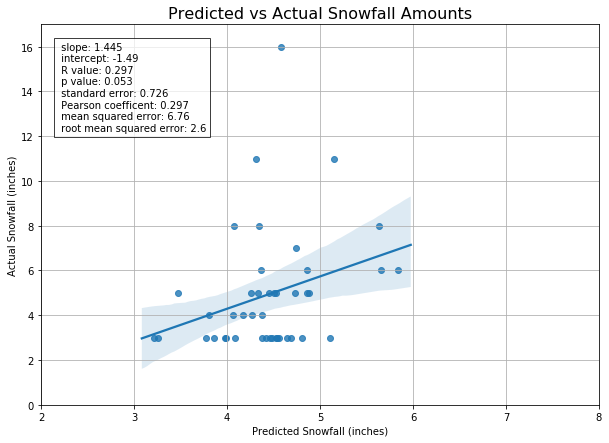
\includegraphics{figs/pred_vs_act_SFC_5c.png} &
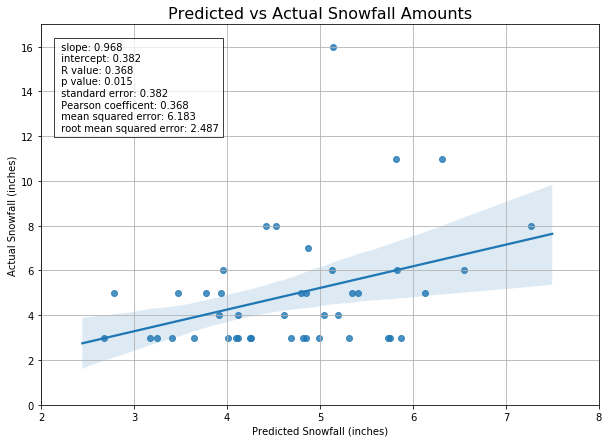
\includegraphics{figs/pred_vs_act_UASFC_6c.png}\tabularnewline
\bottomrule
\end{longtable}

\begin{center}\rule{0.5\linewidth}{\linethickness}\end{center}

\subsubsection{Figure 4- OLS With Partition A: QQ Plot of
Residuals}\label{figure-4--ols-with-partition-a-qq-plot-of-residuals}

\begin{longtable}[]{@{}lc@{}}
\toprule
\textbf{(a) Surface Data Only} & \textbf{(b) Surface Data + Upper Air
Data}\tabularnewline
\midrule
\endhead
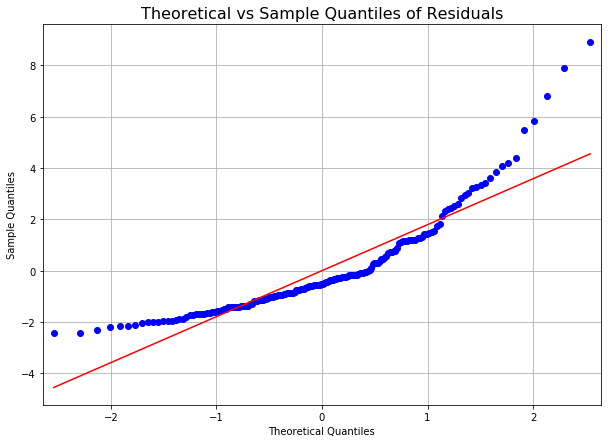
\includegraphics{figs/qq_resid_SFC_5c.png} &
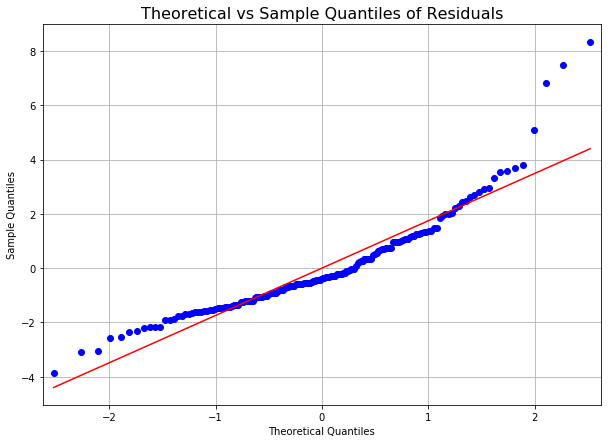
\includegraphics{figs/qq_resid_UASFC_6c.png}\tabularnewline
\bottomrule
\end{longtable}

\begin{center}\rule{0.5\linewidth}{\linethickness}\end{center}

\subsubsection{Figure 5 - OLS With Partition A: Residuals vs Predicted
Snowfall}\label{figure-5---ols-with-partition-a-residuals-vs-predicted-snowfall}

\begin{longtable}[]{@{}lc@{}}
\toprule
\textbf{(a) Surface Data Only} & \textbf{(b) Surface Data + Upper Air
Data}\tabularnewline
\midrule
\endhead
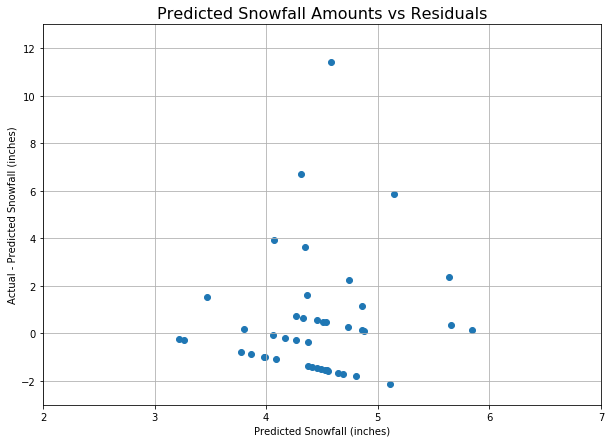
\includegraphics{figs/resid_vs_pred_SFC_5c.png} &
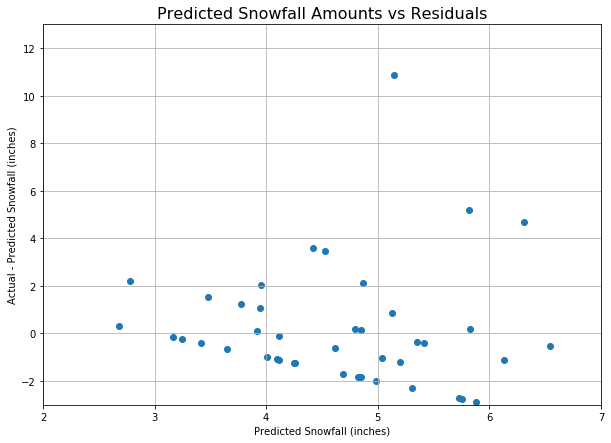
\includegraphics{figs/resid_vs_pred_UASFC_6c.png}\tabularnewline
\bottomrule
\end{longtable}

\begin{center}\rule{0.5\linewidth}{\linethickness}\end{center}

\subsubsection{Figure 6 - OLS With Partition A: Histogram of
Residuals}\label{figure-6---ols-with-partition-a-histogram-of-residuals}

\begin{longtable}[]{@{}lc@{}}
\toprule
\textbf{(a) Surface Data Only} & \textbf{(b) Surface Data + Upper Air
Data}\tabularnewline
\midrule
\endhead
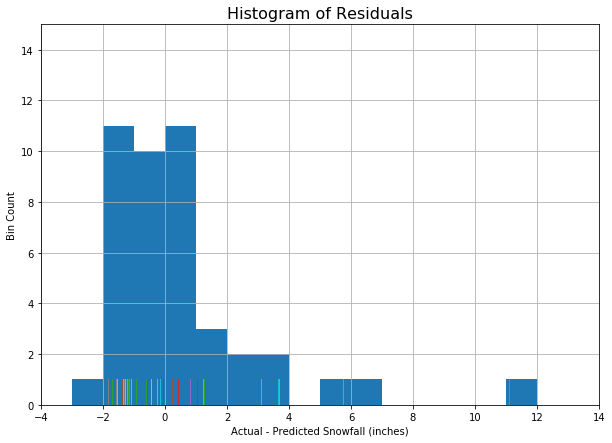
\includegraphics{figs/hist_actual_minus_pred_SFC_5c.png} &
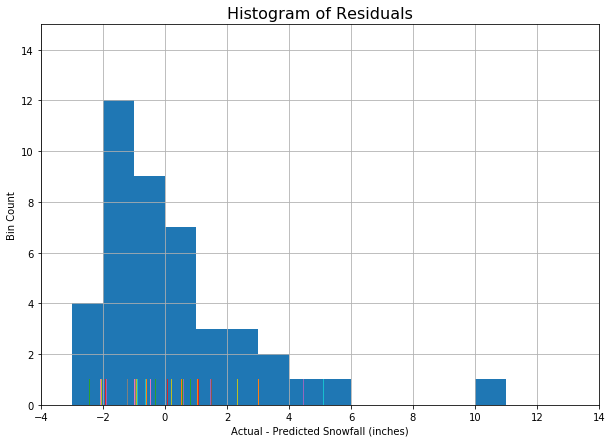
\includegraphics{figs/hist_actual_minus_pred_UASFC_6c.png}\tabularnewline
\bottomrule
\end{longtable}

\section{OLS Model Training/Test Data Partition 2
-\/-\/-\/-\/-\/-\/-\/-\/-\/-\/-\/-\/-\/-\/-\/-\/-\/-\/-\/-\/-\/-\/-\/-\/-\/-\/-\/-\/-\/-\/-\/-\/-\/-\/-\/-\/-\/-\/-\/-\/-\/-\/-\/-\/-\/-\/-\/-\/-\/-\/-\/-\/-\/-\/-\/-\/-\/-\/-\/-\/-\/-\/-\/-\/-\/-\/-\/-\/-\/-\/-\/-\/-\/-\/-\/-\/-\/-\/-\/-\/-\/-\/-\/-\/-\/-\/-\/-\/-\/-\/-\/-\/-\/-\/-\/-\/-\/-\/-\/-\/-\/-\/-\/-\/-\/-\/-\/-\/-}\label{ols-model-trainingtest-data-partition-2--------------------------------------------------------------------------------------------------------------}

\begin{center}\rule{0.5\linewidth}{\linethickness}\end{center}

\begin{center}\rule{0.5\linewidth}{\linethickness}\end{center}

\subsubsection{Figure 7 - OLS With Partition B: Predicted vs Actual
Snowfall
Amounts}\label{figure-7---ols-with-partition-b-predicted-vs-actual-snowfall-amounts}

\begin{longtable}[]{@{}lc@{}}
\toprule
\textbf{(a) Surface Data Only} & \textbf{(b) Surface Data + Upper Air
Data}\tabularnewline
\midrule
\endhead
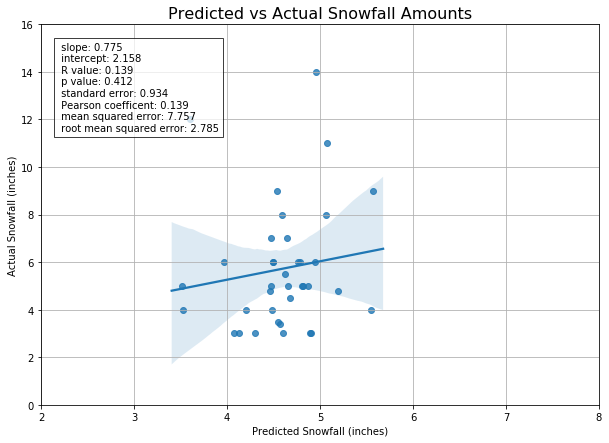
\includegraphics{figs/pred_vs_act_SFC_5d.png} &
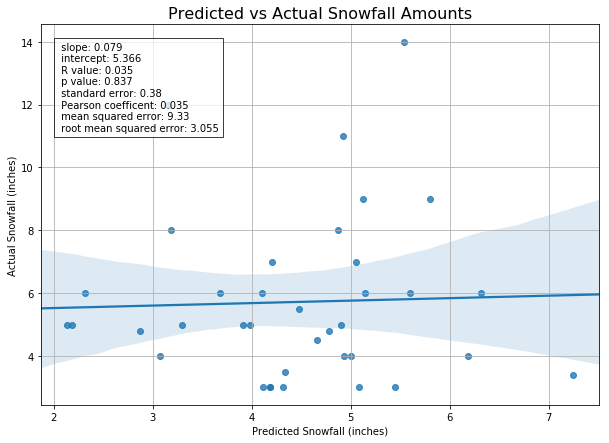
\includegraphics{figs/pred_vs_act_UASFC_6d.png}\tabularnewline
\bottomrule
\end{longtable}

\begin{center}\rule{0.5\linewidth}{\linethickness}\end{center}

\subsubsection{Figure 8- OLS With Partition B: QQ Plot of
Residuals}\label{figure-8--ols-with-partition-b-qq-plot-of-residuals}

\begin{longtable}[]{@{}lc@{}}
\toprule
\textbf{(a) Surface Data Only} & \textbf{(b) Surface Data + Upper Air
Data}\tabularnewline
\midrule
\endhead
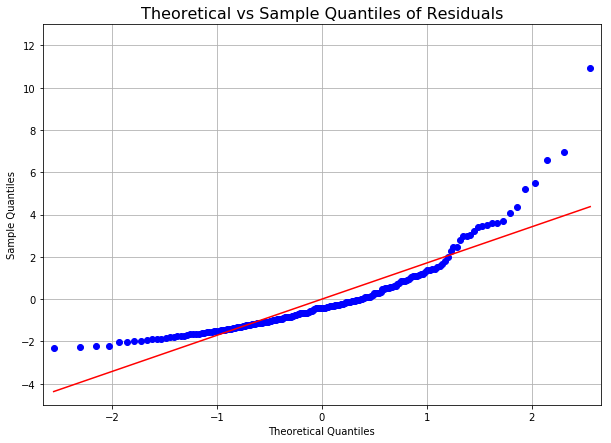
\includegraphics{figs/qq_resid_SFC_5d.png} &
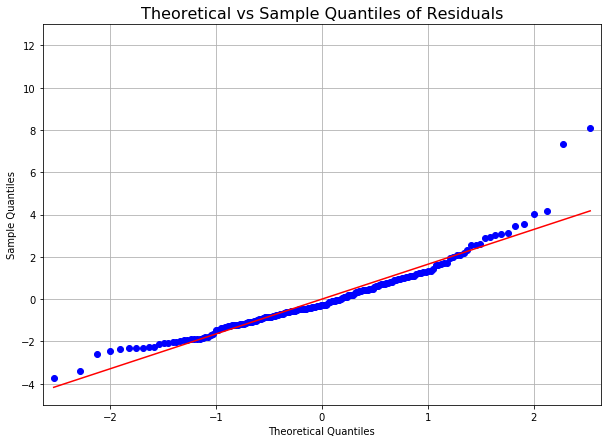
\includegraphics{figs/qq_resid_UASFC_6d.png}\tabularnewline
\bottomrule
\end{longtable}

\begin{center}\rule{0.5\linewidth}{\linethickness}\end{center}

\subsubsection{Figure 9 - OLS With Partition B: Residuals vs Predicted
Snowfall}\label{figure-9---ols-with-partition-b-residuals-vs-predicted-snowfall}

\begin{longtable}[]{@{}lc@{}}
\toprule
\textbf{(a) Surface Data Only} & \textbf{(b) Surface Data + Upper Air
Data}\tabularnewline
\midrule
\endhead
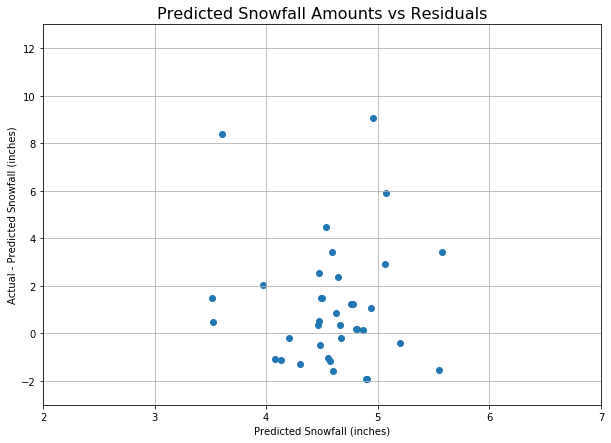
\includegraphics{figs/resid_vs_pred_SFC_5d.png} &
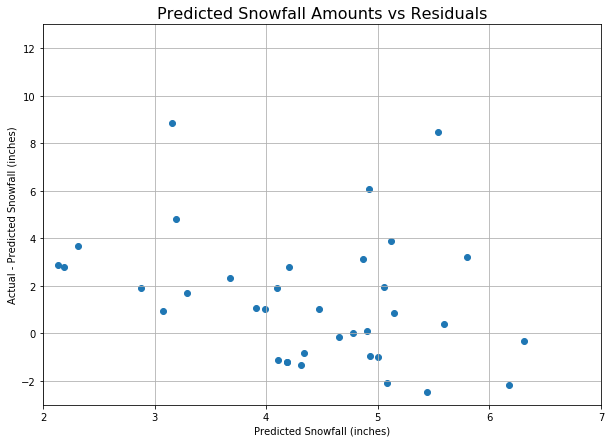
\includegraphics{figs/resid_vs_pred_UASFC_6d.png}\tabularnewline
\bottomrule
\end{longtable}

\begin{center}\rule{0.5\linewidth}{\linethickness}\end{center}

\subsubsection{Figure 10 - OLS With Partition B: Histogram of
Residuals}\label{figure-10---ols-with-partition-b-histogram-of-residuals}

\begin{longtable}[]{@{}lc@{}}
\toprule
\textbf{(a) Surface Data Only} & \textbf{(b) Surface Data + Upper Air
Data}\tabularnewline
\midrule
\endhead
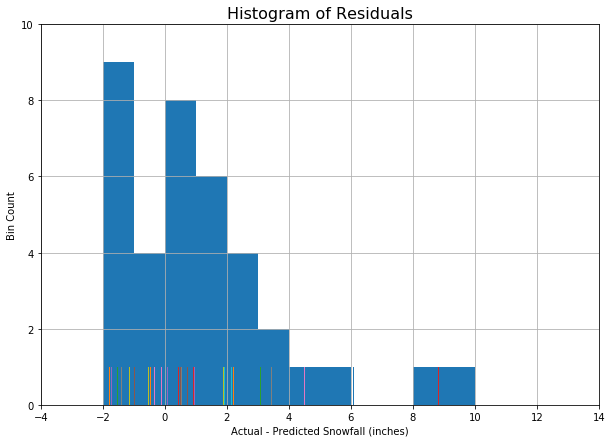
\includegraphics{figs/hist_actual_minus_pred_SFC_5d.png} &
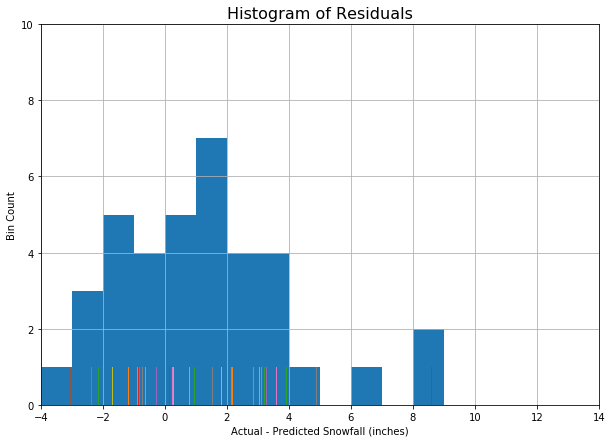
\includegraphics{figs/hist_actual_minus_pred_UASFC_6d.png}\tabularnewline
\bottomrule
\end{longtable}

\section{Cross Validation Using Best Features of Training/Test Data
Partition 1
-\/-\/-\/-\/-\/-\/-\/-\/-\/-\/-\/-\/-\/-\/-\/-\/-\/-\/-\/-\/-\/-\/-\/-\/-\/-\/-\/-\/-\/-\/-\/-\/-\/-\/-\/-\/-\/-\/-\/-\/-\/-\/-\/-\/-\/-\/-\/-\/-\/-\/-\/-\/-\/-\/-\/-\/-\/-\/-\/-\/-\/-\/-\/-\/-\/-\/-\/-\/-\/-\/-\/-\/-\/-\/-\/-\/-\/-\/-\/-\/-\/-\/-\/-\/-\/-\/-\/-\/-\/-\/-\/-\/-\/-\/-\/-\/-\/-\/-\/-\/-\/-\/-\/-\/-\/-\/-\/-\/-}\label{cross-validation-using-best-features-of-trainingtest-data-partition-1--------------------------------------------------------------------------------------------------------------}

\begin{longtable}[]{@{}cc@{}}
\toprule
Surface Data Only & Surface Data + Upper Air Data\tabularnewline
\midrule
\endhead
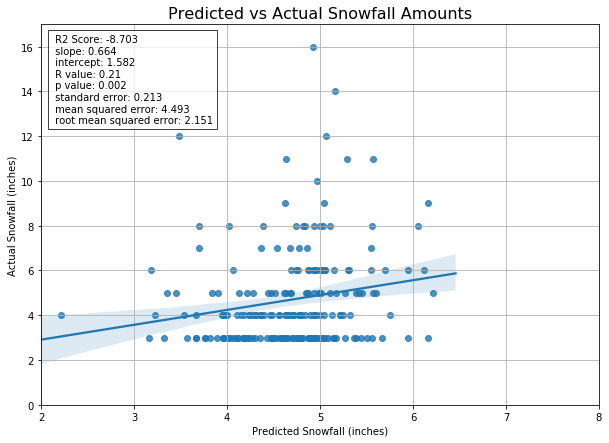
\includegraphics{figs/pred_vs_act_KFold_SFC_P1.png} &
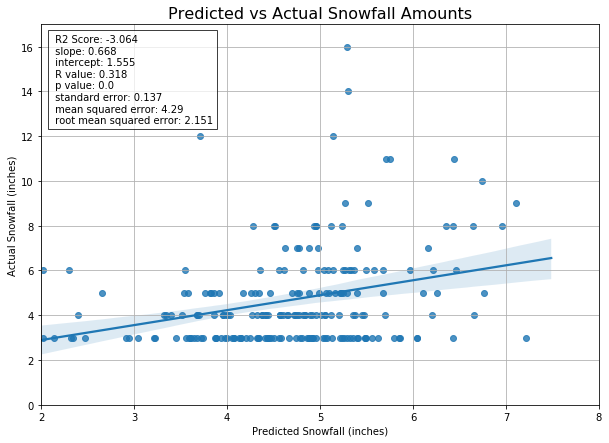
\includegraphics{figs/pred_vs_act_KFold_UASFC_P1.png}\tabularnewline
\bottomrule
\end{longtable}

\begin{center}\rule{0.5\linewidth}{\linethickness}\end{center}

\begin{longtable}[]{@{}lc@{}}
\toprule
Surface Data Only & Surface Data + Upper Air Data\tabularnewline
\midrule
\endhead
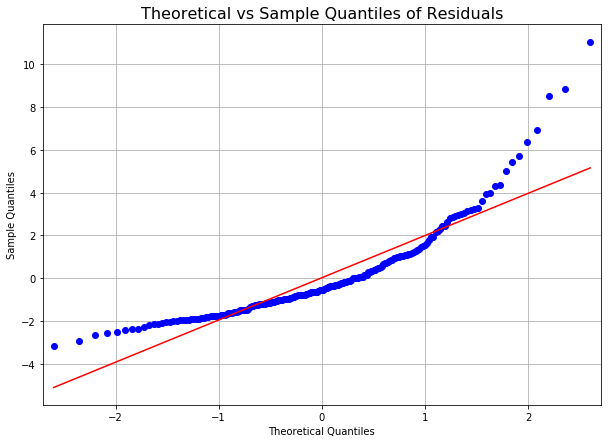
\includegraphics{figs/qq_resid_KFold_SFC_P1.png} &
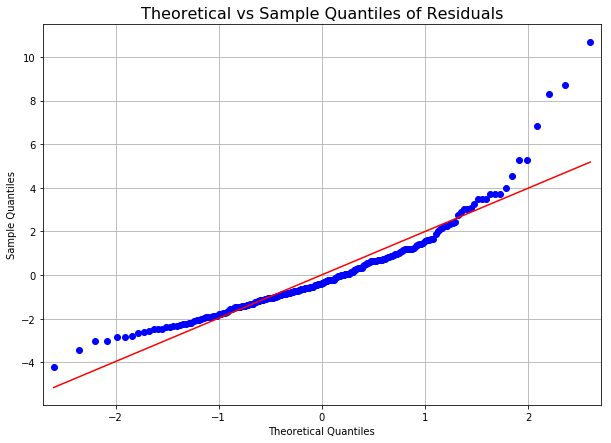
\includegraphics{figs/qq_resid_KFold_UASFC_P1.png}\tabularnewline
\bottomrule
\end{longtable}

\begin{center}\rule{0.5\linewidth}{\linethickness}\end{center}

\begin{longtable}[]{@{}lc@{}}
\toprule
Surface Data Only & Surface Data + Upper Air Data\tabularnewline
\midrule
\endhead
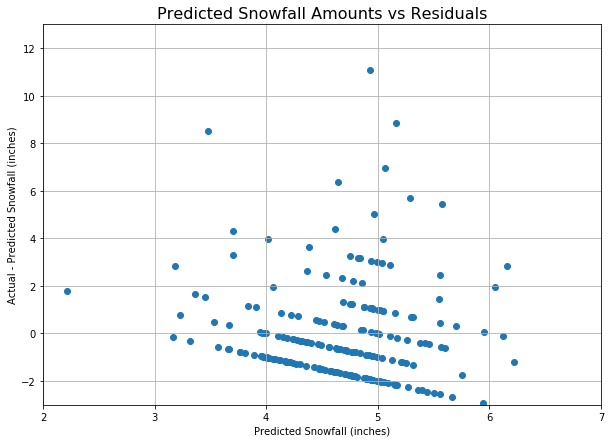
\includegraphics{figs/resid_vs_pred_KFold_SFC_P1.png} &
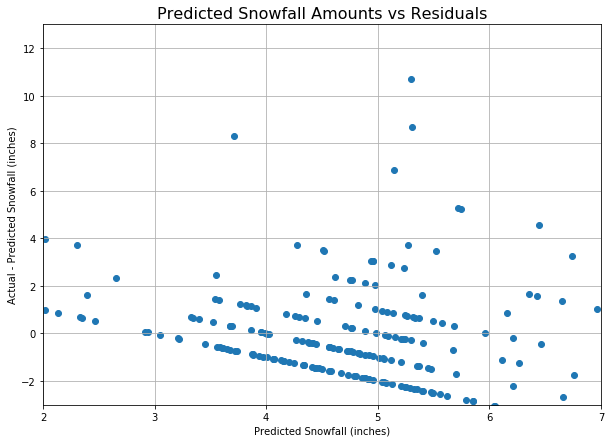
\includegraphics{figs/resid_vs_pred_KFold_UASFC_P1.png}\tabularnewline
\bottomrule
\end{longtable}

\begin{center}\rule{0.5\linewidth}{\linethickness}\end{center}

\begin{longtable}[]{@{}lc@{}}
\toprule
Surface Data Only & Surface Data + Upper Air Data\tabularnewline
\midrule
\endhead
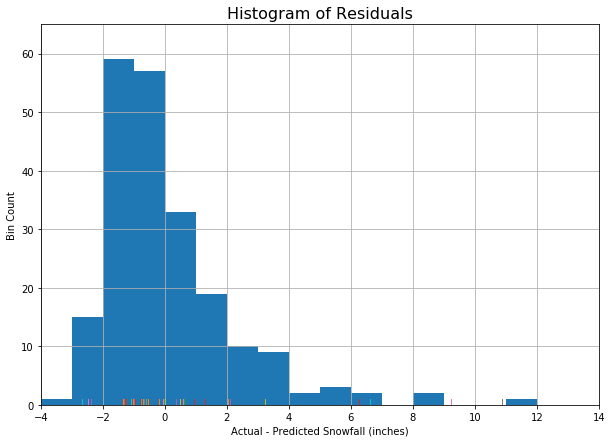
\includegraphics{figs/hist_actual_minus_pred_KFold_SFC_P1.png} &
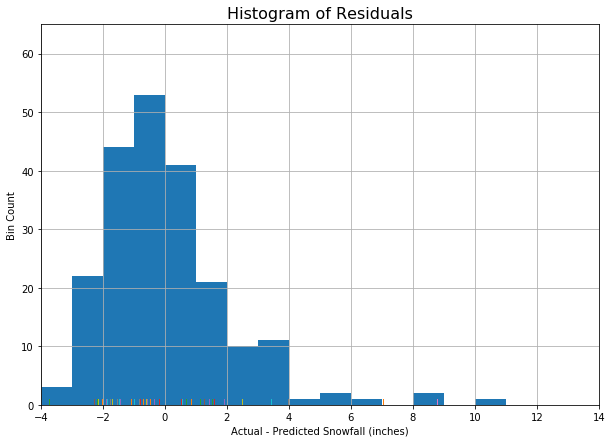
\includegraphics{figs/hist_actual_minus_pred_KFold_UASFC_P1.png}\tabularnewline
\bottomrule
\end{longtable}

\section{Cross Validation Using Best Features of Training/Test Data
Partition 2
-\/-\/-\/-\/-\/-\/-\/-\/-\/-\/-\/-\/-\/-\/-\/-\/-\/-\/-\/-\/-\/-\/-\/-\/-\/-\/-\/-\/-\/-\/-\/-\/-\/-\/-\/-\/-\/-\/-\/-\/-\/-\/-\/-\/-\/-\/-\/-\/-\/-\/-\/-\/-\/-\/-\/-\/-\/-\/-\/-\/-\/-\/-\/-\/-\/-\/-\/-\/-\/-\/-\/-\/-\/-\/-\/-\/-\/-\/-\/-\/-\/-\/-\/-\/-\/-\/-\/-\/-\/-\/-\/-\/-\/-\/-\/-\/-\/-\/-\/-\/-\/-\/-\/-\/-\/-\/-\/-\/-}\label{cross-validation-using-best-features-of-trainingtest-data-partition-2--------------------------------------------------------------------------------------------------------------}

\begin{longtable}[]{@{}lc@{}}
\toprule
Surface Data Only & Surface Data + Upper Air Data\tabularnewline
\midrule
\endhead
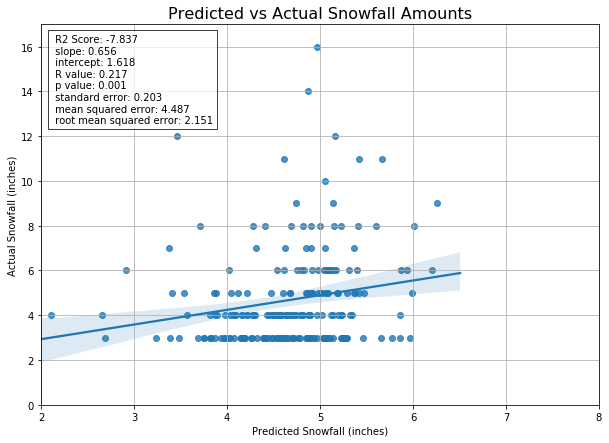
\includegraphics{figs/pred_vs_act_KFold_SFC_P2.png} &
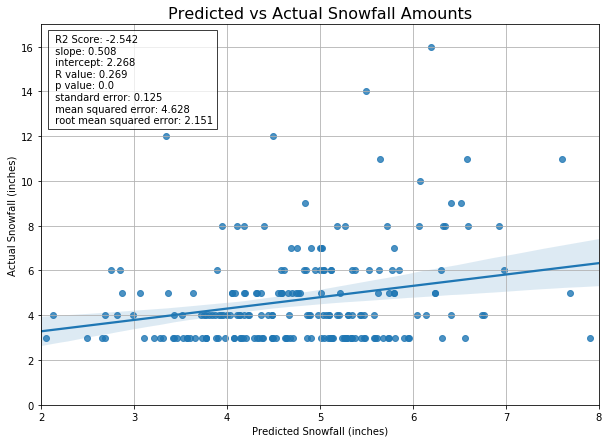
\includegraphics{figs/pred_vs_act_KFold_UASFC_P2.png}\tabularnewline
\bottomrule
\end{longtable}

\begin{center}\rule{0.5\linewidth}{\linethickness}\end{center}

\begin{longtable}[]{@{}lc@{}}
\toprule
Surface Data Only & Surface Data + Upper Air Data\tabularnewline
\midrule
\endhead
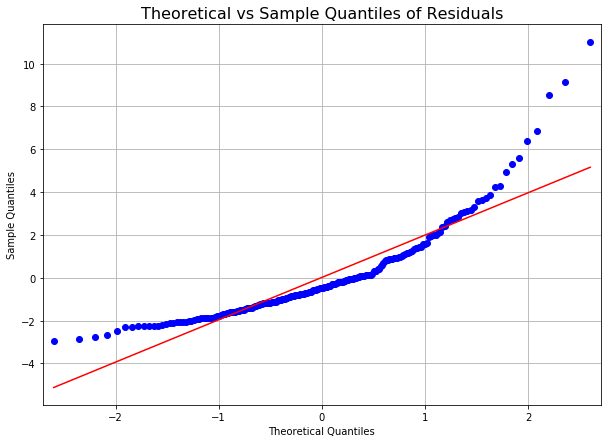
\includegraphics{figs/qq_resid_KFold_SFC_P2.png} &
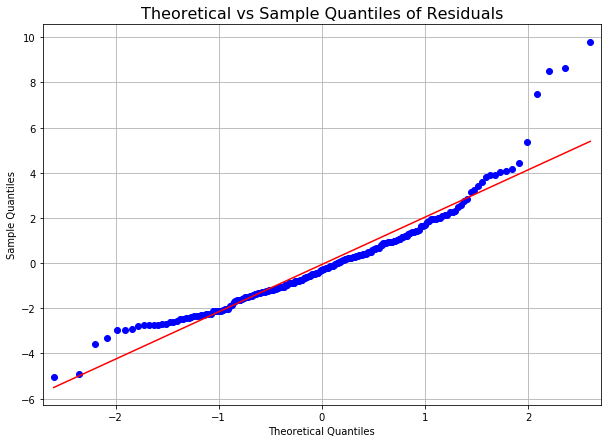
\includegraphics{figs/qq_resid_KFold_UASFC_P2.png}\tabularnewline
\bottomrule
\end{longtable}

\begin{center}\rule{0.5\linewidth}{\linethickness}\end{center}

\begin{longtable}[]{@{}lc@{}}
\toprule
Surface Data Only & Surface Data + Upper Air Data\tabularnewline
\midrule
\endhead
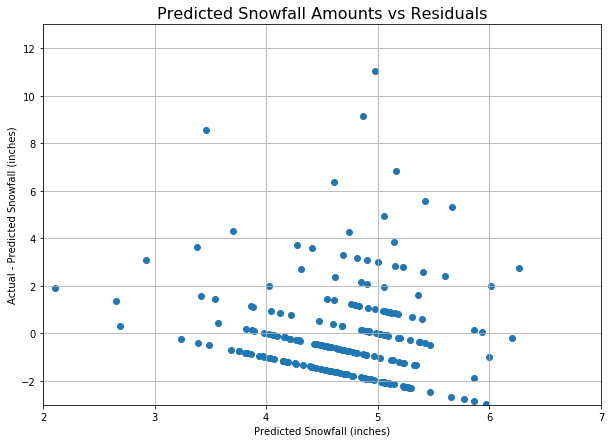
\includegraphics{figs/resid_vs_pred_KFold_SFC_P2.png} &
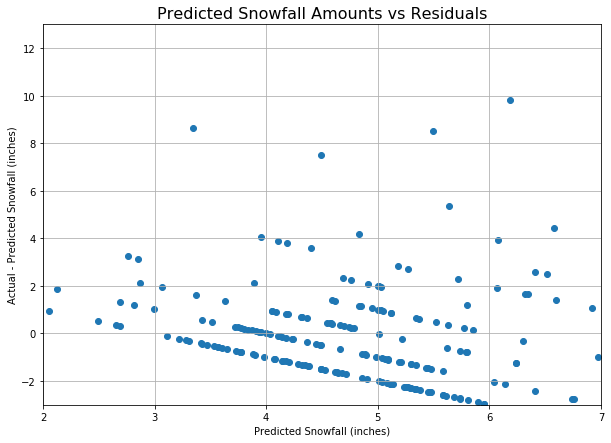
\includegraphics{figs/resid_vs_pred_KFold_UASFC_P2.png}\tabularnewline
\bottomrule
\end{longtable}

\begin{center}\rule{0.5\linewidth}{\linethickness}\end{center}

\begin{longtable}[]{@{}lc@{}}
\toprule
Surface Data Only & Surface Data + Upper Air Data\tabularnewline
\midrule
\endhead
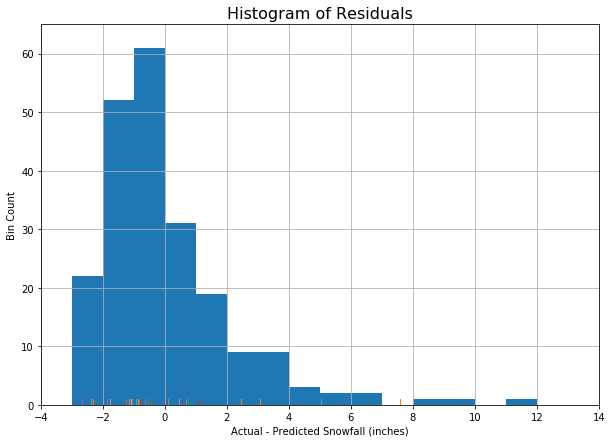
\includegraphics{figs/hist_actual_minus_pred_KFold_SFC_P2.png} &
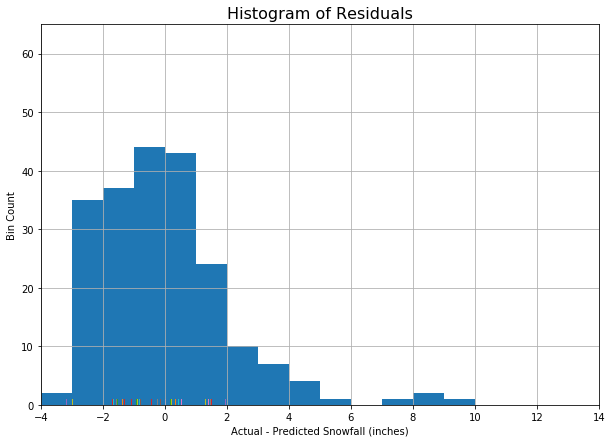
\includegraphics{figs/hist_actual_minus_pred_KFold_UASFC_P2.png}\tabularnewline
\bottomrule
\end{longtable}

\subsubsection{Surface Data Only}\label{surface-data-only}

\subsubsection{Surface + Upper Air Data}\label{surface-upper-air-data}

\subsection{Decision Tree Regressor
Model}\label{decision-tree-regressor-model}

\subsection{Conclusion}\label{conclusion}

While not large, there are some significant relationships between some
meteorological variables and snowfall amount when snowfall does occur.
It is anticipated that there may be some 12-hr snowfall predictive
ability predicting snowfall utilizing a very simple Ordinary Least
Squares model with only meteorological measurements - especially
dewpoint and 12-hr pressure changes. There is recognition that snowfall
is a very complex variable to forecast, and a simple OLS model may have
limitations. Snowfall amounts can dependent on a variety of factors
including snow water equivalent, temperature during crystal formation in
the upper atmosphere, along with melting/freezing activity as snowflakes
fall to the surface. Upper air data may be helpful in overcoming some of
these complexities and limitations, and my be integrated in this
analysis. Despite the complexities of a snowfall prediction, an OLS
model is a good starting point to begin to understand how data science
techniques could be utilized.

\section{Decision Tree
-\/-\/-\/-\/-\/-\/-\/-\/-\/-\/-\/-\/-\/-\/-\/-\/-\/-\/-\/-\/-\/-\/-\/-\/-\/-\/-\/-\/-\/-\/-\/-\/-\/-\/-\/-\/-\/-\/-\/-\/-\/-\/-\/-\/-\/-\/-\/-\/-\/-\/-\/-\/-\/-\/-\/-\/-\/-\/-\/-\/-\/-\/-\/-\/-\/-\/-\/-\/-\/-\/-\/-\/-\/-\/-\/-\/-\/-\/-\/-\/-\/-\/-\/-}\label{decision-tree-------------------------------------------------------------------------------------}

\begin{longtable}[]{@{}lc@{}}
\toprule
Surface Data Only & Surface Data + Upper Air Data\tabularnewline
\midrule
\endhead
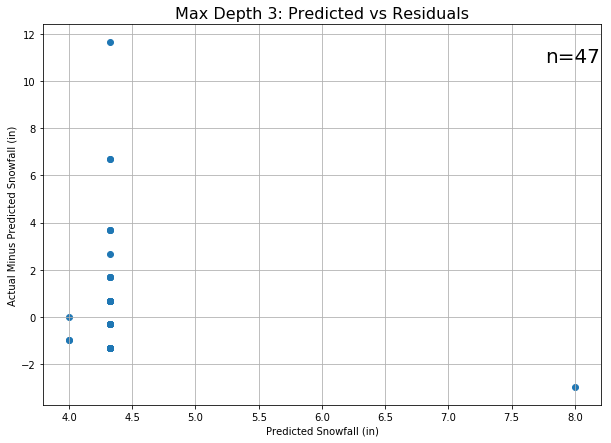
\includegraphics{figs/TREE_pred_vs_residuals_SFC.png} &
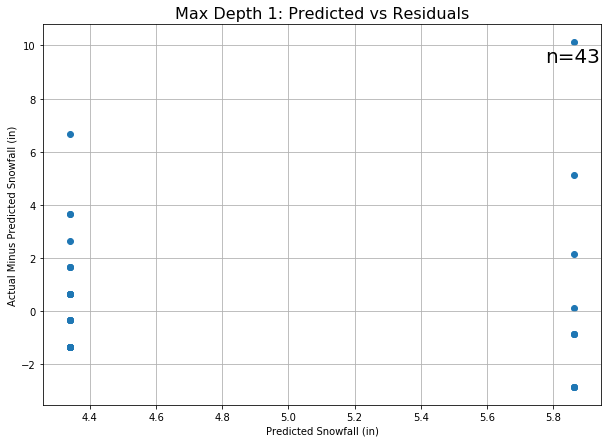
\includegraphics{figs/TREE_pred_vs_residuals_UASFC.png}\tabularnewline
\bottomrule
\end{longtable}

\begin{center}\rule{0.5\linewidth}{\linethickness}\end{center}

\begin{longtable}[]{@{}lc@{}}
\toprule
Surface Data Only & Surface Data + Upper Air Data\tabularnewline
\midrule
\endhead
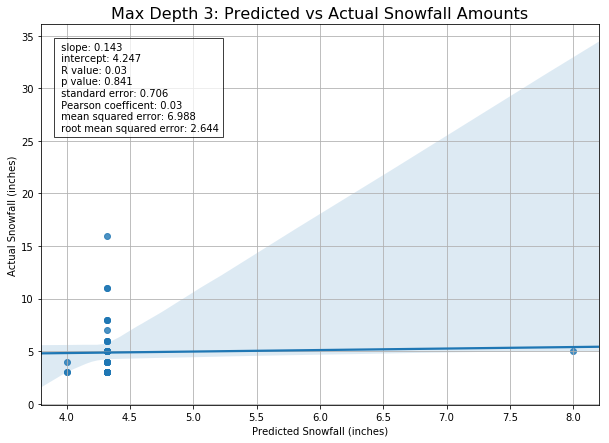
\includegraphics{figs/TREE_pred_vs_act_SFC.png} &
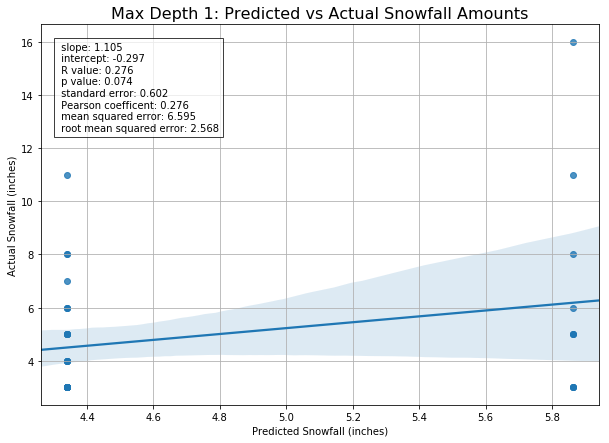
\includegraphics{figs/TREE_pred_vs_act_UASFC.png}\tabularnewline
\bottomrule
\end{longtable}

\begin{center}\rule{0.5\linewidth}{\linethickness}\end{center}

\begin{longtable}[]{@{}lc@{}}
\toprule
Surface Data Only & Surface Data + Upper Air Data\tabularnewline
\midrule
\endhead
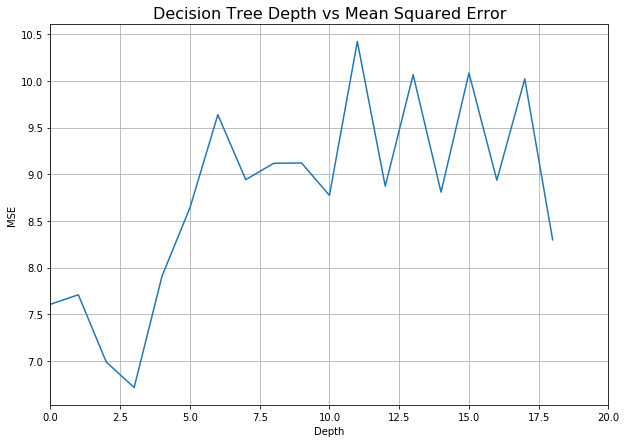
\includegraphics{figs/TREE_depth_vs_mse_SFC.png} &
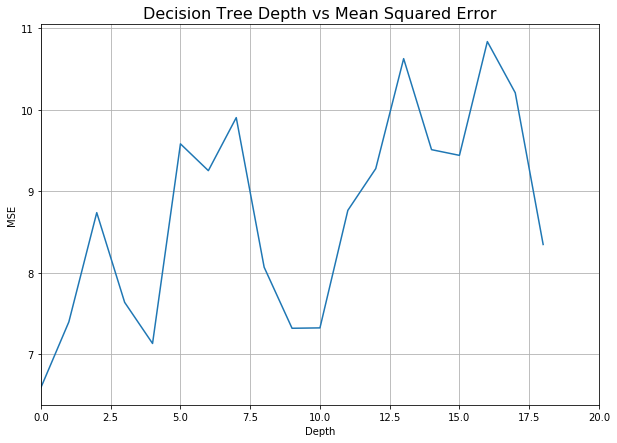
\includegraphics{figs/TREE_depth_vs_mse_UASFC.png}\tabularnewline
\bottomrule
\end{longtable}

\textbf{Surface Data Only Decision Tree}

\begin{figure}
\centering
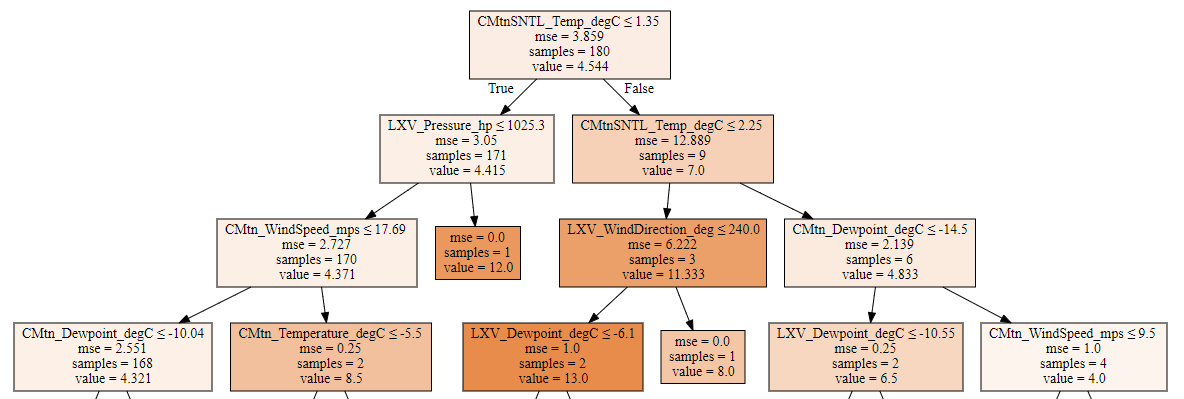
\includegraphics{figs/TREE_DecisionTree_SFC.png}
\caption{}
\end{figure}

\begin{center}\rule{0.5\linewidth}{\linethickness}\end{center}

\textbf{Surface + Upper Air Data Decision Tree}

\begin{figure}
\centering
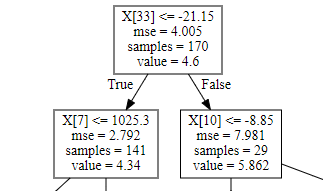
\includegraphics{figs/TREE_DecisionTree_UASFC.png}
\caption{}
\end{figure}

\section{Decision Tree
-\/-\/-\/-\/-\/-\/-\/-\/-\/-\/-\/-\/-\/-\/-\/-\/-\/-\/-\/-\/-\/-\/-\/-\/-\/-\/-\/-\/-\/-\/-\/-\/-\/-\/-\/-\/-\/-\/-\/-\/-\/-\/-\/-\/-\/-\/-\/-\/-\/-\/-\/-\/-\/-\/-\/-\/-\/-\/-\/-\/-\/-\/-\/-\/-\/-\/-\/-\/-\/-\/-\/-\/-\/-\/-\/-\/-\/-\/-\/-\/-\/-\/-\/-}\label{decision-tree--------------------------------------------------------------------------------------1}

\begin{longtable}[]{@{}lc@{}}
\toprule
Surface Data Only & Surface Data + Upper Air Data\tabularnewline
\midrule
\endhead
\includegraphics{figs/TREE_pred_vs_residuals_SFC_5c.png} &
\includegraphics{figs/TREE_pred_vs_residuals_UASFC_5c.png}\tabularnewline
\bottomrule
\end{longtable}

\begin{center}\rule{0.5\linewidth}{\linethickness}\end{center}

\begin{longtable}[]{@{}lc@{}}
\toprule
Surface Data Only & Surface Data + Upper Air Data\tabularnewline
\midrule
\endhead
\includegraphics{figs/TREE_pred_vs_act_SFC_5c.png} &
\includegraphics{figs/TREE_pred_vs_act_UASFC_5c.png}\tabularnewline
\bottomrule
\end{longtable}

\begin{center}\rule{0.5\linewidth}{\linethickness}\end{center}

\begin{longtable}[]{@{}lc@{}}
\toprule
Surface Data Only & Surface Data + Upper Air Data\tabularnewline
\midrule
\endhead
\includegraphics{figs/TREE_depth_vs_mse_SFC_5c.png} &
\includegraphics{figs/TREE_depth_vs_mse_UASFC_5c.png}\tabularnewline
\bottomrule
\end{longtable}

\begin{center}\rule{0.5\linewidth}{\linethickness}\end{center}

\begin{center}\rule{0.5\linewidth}{\linethickness}\end{center}


    % Add a bibliography block to the postdoc
    
    
    
    \end{document}
